\documentclass[a4paper,12pt,oneside]{book}
\usepackage{latexsym}
\usepackage{braket}
\usepackage{graphicx}
\usepackage{amsfonts}
\usepackage{amsmath}
\usepackage{verbatim}
\usepackage{amssymb}
\usepackage{amsthm}
\usepackage{graphicx}
\usepackage[english]{babel}
\usepackage[utf8]{inputenc}
\usepackage{listings}
\usepackage{color}
\usepackage{float}
\usepackage{geometry}
\usepackage{algorithm}
\usepackage{algpseudocode}
\usepackage{pdfpages}


%\usepackage[colorlinks]{hyperref}
%\hypersetup{urlcolor=darkblue}

\pagestyle{plain}

\lstset{
  basicstyle=\ttfamily,
  columns=fullflexible,
  showstringspaces=false,
  commentstyle=\color{gray}\upshape
}

\definecolor{darkblue}{rgb}{0.0,0.0,0.8}
\definecolor{green}{rgb}{0,0.6,0}
\definecolor{gray}{rgb}{0.5,0.5,0.5}
\definecolor{darkgray}{rgb}{0.105,0.105,0.105}
\definecolor{mauve}{rgb}{0.58,0,0.82}
\definecolor{black}{rgb}{0,0,0}
\definecolor{purple}{rgb}{0.72,0.61,0.139}
%\definecolor{ocra}{rgb}{0.204, 0.119, 0.34}
\definecolor{ocra}{rgb}{0.184,0.134,0.11}
\definecolor{maroon}{rgb}{0.5,0,0}
\definecolor{darkgreen}{rgb}{0,0.5,0}

\lstdefinelanguage{XML}
{
  basicstyle=\ttfamily,
  morestring=[s]{"}{"},
  morecomment=[s]{?}{?},
  morecomment=[s]{!--}{--},
  commentstyle=\color{darkgreen},
  moredelim=[s][\color{black}]{>}{<},
  moredelim=[s][\color{red}]{\ }{=},
  stringstyle=\color{blue},
  identifierstyle=\color{maroon}
}

\lstdefinelanguage{CCC}{ 
  breakatwhitespace=false,         
  breaklines=true,                 
  captionpos=b,                   
  frame=single,                    
  keepspaces=true,                 
  numbers=left,                    
  numbersep=5pt,                   
  numberstyle=\tiny\color{gray}, 
  rulecolor=\color{black},         
  showtabs=false,                  
  stepnumber=1,                    
  tabsize=2,                       
  title=\lstname,                   
 language=C++,
 basicstyle=\ttfamily,
 morekeywords={A}, 
 keywordstyle=\color{darkblue}\ttfamily,
 %identifierstyle=\color{green},
 stringstyle=\color{red}\ttfamily,
 %numberstyle=\color{purple}
 commentstyle=\color{gray}\ttfamily,
 morecomment=[l][\color{mauve}]{\#}
}

\lstdefinelanguage{AST}{ 
  breakatwhitespace=false,         
  breaklines=true,                 
  captionpos=b,                   
  frame=single,                   
  keepspaces=true,                 
  rulecolor=\color{black},         
  showtabs=false,                  
  tabsize=2,                       
  title=\lstname,                   
  morekeywords={A}, 
  keywordstyle=\color{black},
 language=C++,
  %identifierstyle=\color{green},
  stringstyle=\color{ocra},
  %numberstyle=\color{purple},
 basicstyle=\color{gray}\scriptsize
}
\renewcommand{\lstlistingname}{Code}
\geometry{left=4cm}
\geometry{right=2cm}
\linespread{1.1}
\author{Giacomo Dabisias, Filippo Brizzi}
\title{A framework for static allocation of parallel OpenMp code on multi-core platforms}
\frenchspacing

\begin{document}
\frontmatter
\tableofcontents

\chapter{Abstract}

The aim of this thesis is to create a framework for guaranteeing \emph{real-time} constraints on parallel \emph{OpenMP} C++ code. The framework provides a static schedule for the allocation of tasks on system threads and a run-time support for the \emph{real-time} execution. In order to do so the original source code is first instrumented, then profiled and finally rewritten by means of clang. Performance results are provided on a Computer Vision application.

\section{Chapter's structure}

\mainmatter
\chapter{Introduction}

\section{Motivation, context and target application}

The last years have seen the transition from single core architectures towards multicore architectures, mainly in the desktop and server enviroment. Lately also small devices as smartphones, embedded microprocessors and tablets have started to use more than a single core processor. The actual trend is to use a lot of cores with just a reduced instruction set as in \emph{general purpose GPUs}.

\emph{Real time} systems are becoming more and more common, finding their place in almost all aspects of our daily routines; this systems often consist of several applications executing concurrently on shared resources. 
The main differences between these systems and a system designed to achive high performance can be summarized as follows:
\begin{itemize}
\item{ \emph{real time} programs need strict timing guarantees, while high performance programs try to achive the lowest possible computation time, usually in a best effort manner.}
\item{\emph{Real time} programs need to be predictable; in principle it could be that a real time program could finish almost always before its deadline on a high performance system, but it could be that in some exceptional cases, due to execution preemption, context switches, concurrent resource access \dots the program does not finish in time. To solve this, it may happen that the mean execution time of the real time program grows, but the program becomes also predictable, in the sense that it always finishes within its deadline.}
\item{ High performance systems need to "scale" well when the architecture becomes more powerful, while \emph{real time} systems need just to satisfy the timing contrains, even with no performance gain.}

\end{itemize}

The most relevant drawback of actual real time systems is that most of them are usually made to exploit just one single computing core, while their capabilities demand is growing. Applications like Computer Vision, Robotics, Simulation, Video Encoding/Decoding, Software Defined Radios, \dots have the necessity to process in parallel more tasks to achive a positive feedback for the user. This brings two possible solutions:
\begin{itemize}
\item{find new and better scheduling algorithms to allocate new tasks using the same single core architecture.}
\item{Upgrade the processing power by adding new computing cores or by using a faster single core.}
\end{itemize}

The first solution has the disadvantage that, if the computing resources are already perfectly allocated, it is not possible to find any better scheduling for the tasks to make space for a new job. A faster single core is also often not feasible, given the higher power consumption and temperature; this aspect is very relevant in embedded devices. 
The natural solution to the problem is to exploit the new trend toward multicore systems; this solution has opened a new research field and has brought to view a lot of new challenging problems. Given that the number of cores is doubling according to the well known \emph{Moores law}, it is very important to find a fast and architecture independent way to map a set of \emph{real time} tasks on computing cores. With such a tool, it would be possible to upgrade or change the computing architecture in case of new \emph{real time} jobs, just scheduling them on the new system.

There is plenty of works on the problem of scheduling \emph{real time} tasks on multiprocesses, but they are all mainly theoretical \cite{bbw2}\cite{real1}\cite{real2}.



\section{Objectives}

The described tool aims to solve the previously stated problems providing the following features.

\begin{itemize}
\item{an easy \emph{API} for the programmer to specify the concurrency between \emph{real time} tasks together with all the necessary scheduling parameters (deadlines, computation times, activation times \dots)}
\item{A way to visualize task concurrency and code structure as graphs.}
\item{A \emph{scheduling algorithm} which supports multicore architectures, adapting to the specific platform.}
\item{A \emph{run time support} for the program execution which guarantees the scheduling order of tasks and their timing contrains.}
\end{itemize}


\section{Supporting parallelism in C/C++}

In the last years the diffusion of multi-core platforms has rapidly increased enhancing the need of tools and libraries to write multi-threaded programs. 

Several major software companies developed their own multi-thread libraries like Intel with Thread Building Block (TBB) \cite{tbb} and Microsoft with Parallel Patterns Library (PPL) \cite{ppl}. There are also several open-source libraries like Boost \cite{boost} and OpenMP \cite{openmp}. With the release of C++11 standard also the standard C++ library supports threading.

Lately appeared also automatic parallelization tools; these softwares allow to automatically transform a sequential code into an equivalent parallel one, like the Intel C++ compiler \cite{icc} and Parallware \cite{parallware}.  

Lastly it is worth to mention briefly GPUs, that have become accessible to programmers with the release of tools like Nvidia's CUDA or the open-source OpenCL. These libraries allow the user to easily run code on the GPU; of course the program to run must have some particular features because GPU are still not general purpose. 

It was necessary to find two multi-threaded libraries, one used by the input program to describe its parallel sections and the other to run the input program with the static custom schedule, in described framework.

The first library has to satisfy the following requirements: it has to allow to transform easily a given sequential \emph{real-time} code into a parallel one, without upsetting too much the original structure of the code, given that these kind of code have been usually deeply tested and must meet strict requirements.

What stated above is also crucial since one of the steps of the tool is to extract informations from the parallel code, such as the differences between two parallels regions of code and their precedences and dependencies. These informations are fundamental to be able to transform the code in a set of tasks and to provide to the schedule algorithm the most accurate parameters. Furthermore the parallel code has to be instrumented both to profile it and to divide it into tasks for the final execution. The analysis of the various libraries didn’t focus on their execution performance as the aim of the tool is to use the library calls just to get the structure of the parallel code.

\emph{OpenMP} resulted as the best choice and its behaviour is described in full details in chapter~\ref{openmp}. The main motivations that brought to this decision are the following. First of all  \emph{OpenMP} has a minimal code overhead since it just adds annotations inside the original sequential code, without any needs of changing its structure.  \emph{OpenMP} works embedding pieces of code inside C++ scopes and adding annotations to each of these scopes by mean of pragma constructs. The scopes automatically identify the distinct code blocks (tasks) and also give immediately some information about the dependencies among them. The use of pragmas is very convenient as they are skipped by the compiler if not informed with a specific flag. This implies that, given an  \emph{OpenMP} code, to run it sequentially is just enough to not inform the compiler of the presence of  \emph{OpenMP}; this feature will be usefull to profile the code.  \emph{OpenMP} is well supported by the main compilers and it has a strong and large develop community, including big companies such as Intel and IBM. \emph{OpenMP} has already been used as support to simulate tasks structure for a parallel scheduling algorithm in \cite{realtimeopenmp}. Here the authors analyze the problem of scheduling periodic real-time tasks on multiprocessors under the fork-join structure used in \emph{OpenMP}; the article produces just theoretical results.

The second library has instead opposite requirements as it has to be highly efficient; for this reason the C++ standard library has been chosen. Since the release of C++11 standard, the C++ standard library was provided with threads, mutexes, semaphores and condition variables. This library has the drawback of being not easy to use when coming to complicated and structured tasks, but on the other hand it is fully customizable as it allows to instantiate and use directly system threads. It provides the chance to directly tune the performance of the whole program and it allows to allocate each task on a specific thread, unlike the other parallelization tools.

\section{The OpenMP standard}
\label{openmp}

Jointly defined by a group of major computer hardware and software vendors, \emph{OpenMP} is a portable, scalable model that gives shared-memory parallel programmers a simple and flexible interface for developing parallel applications for platforms ranging from desktops to supercomputers.

The \emph{OpenMP API} uses the fork-join model of parallel execution. Multiple threads of execution perform tasks defined implicitly or explicitly by \emph{OpenMP} directives. The \emph{OpenMP API} is intended to support programs that will execute correctly both as parallel programs (multiple threads of execution and a full \emph{OpenMP} support library) and as sequential programs (directives ignored and a simple \emph{OpenMP} stubs library).

An \emph{OpenMP} program begins as a single thread of execution, called an initial thread. An initial thread executes sequentially, as if enclosed in an implicit task region, called an initial task region that is defined by the implicit parallel region surrounding the whole program.

If a construct creates a data environment after an \emph{OpenMP} directive, the data environment is created at the time the construct is encountered. Whether a construct creates a data environment is defined in the description of the construct. When any thread encounters a parallel construct, the thread creates a team of itself and zero or more additional threads and becomes the master of the new team. The code for each task is defined by the code inside the parallel construct. Each task is assigned to a different thread in the team and becomes tied; that is, it is always executed by the thread to which it is initially assigned. The task region of the task being executed by the encountering thread is suspended, and each member of the new team executes its implicit task. Each directive uses a number of threads defined by the standard or it can be set using the function call \emph{void omp\_set\_num\_threads(int num\_threads)}. In this project this call is not allowed and the thread number for each directive is managed separately. There is an implicit barrier at the end of each parallel construct; only the master thread resumes execution beyond the end of the parallel construct, resuming the task region that was suspended upon encountering it. Any number of parallel constructs can be specified in a single program. 

It is very important to notice that \emph{OpenMP}-compliant implementations are not required to check for data dependencies, data conflicts, race conditions, or deadlocks, any of which may occur in conforming programs. In addition, compliant implementations are not required to check for code sequences that cause a program to be classified as non conforming. Also the developed tool will only accept well written programs, whitout checking if they are \emph{OpenMP}-compliant. The \emph{OpenMP} specification makes also no guarantee that input or output to the same file is synchronous when executed in parallel. In this case, the programmer is responsible for synchronizing input and output statements (or routines) using the provided synchronization constructs or library routines; this assumption is also maintained in the developed tool.

In C/C++, \emph{OpenMP} directives are specified by using the\begin{bf} $\#$pragma\end{bf} mechanism provided by the C and C++ standards.  Almost all directives start with \begin{bf}$\#$pragma omp\end{bf} and have the following grammar:
\begin{bf}{\center{$\#$pragma omp directive-name [clause[ [,] clause]...] new-line}}\end{bf}
\\

A directive applies to at most one succeeding statement, which must be a structured block, and may be composed of consecutive $\#$pragma preprocessing directives. 

It is possible to specify for each variable, in an \emph{OpenMP} directive, if it should be private or shared by the threads; this can be done using the clause attribute \emph{shared(variable)} or \emph{private(variable)}.

There is a big variety of directives which permit to express almost all computational patterns; for this reason a restricted set has been choosen in this project. \emph{Real-time} applications tend to be composed by a lot of small jobs, with only a small amount of shared variables and a lot of controllers. Given this, the following \emph{OpenMP} directives have been choosen:
\begin{itemize}
\item{\begin{bf}{$\#$pragma omp parallel}\end{bf} : all the code inside of this block is executed in parallel by all the available threads. Each thread has its own variables scope defined by the appropriate clauses. }
\item{\begin{bf}{$\#$pragma omp sections}\end{bf} : this pragma opens a block which has to contain section directives; it has always to be contained inside a \begin{bf}$\#$pragma omp parallel block\end{bf} and there is an implicit barrier at the end of this block synchronizing all the \emph{section} blocks which are included. }
\item{\begin{bf}{$\#$pragma omp section}\end{bf} : all the code inside of this block is executed in parallel by only \emph{one} thread. }
\item{\begin{bf}{$\#$pragma omp for}\end{bf} : this pragma must precede a for cycle. In this case the \emph{for loop} is splitted among  threads and a private copy of the looping variable is associated to each. This pragma must be nested in a \begin{bf}$\#$pragma omp parallel\end{bf} directive or can be expressed as \begin{bf}{$\#$pragma omp parallel for}\end{bf} without the need of the previous one.  }
\item{\begin{bf}{$\#$pragma single}\end{bf} : this pragma must be nested inside a \begin{bf}{$\#$pragma omp parallel }\end{bf} and means that the code block contained in it must be executed only by a single thread.}
\item{\begin{bf}{$\#$pragma task}\end{bf} : this pragma must be nested inside a \begin{bf}{$\#$pragma omp parallel }\end{bf} and means that all the possible threads will execute in parallel the same code block contained in it. In the developed tool this structure is not allowed. The allowed structure instead is composed by a number of \begin{bf}{$\#$pragma task}\end{bf} nested inside a \begin{bf}{$\#$pragma single}\end{bf} block. The semantic of this contruct is the same as  having \begin{bf}{$\#$pragma omp section}\end{bf}s inside \begin{bf}{$\#$pragma omp sections}\end{bf}.}
\end{itemize}
The considered pragma set can be splitted into two groups: 
\begin{itemize}
\item{a first set composed of \begin{bf}{$\#$pragma omp parallel}\end{bf}, \begin{bf}{$\#$pragma omp sections}\end{bf} and \begin{bf}{ $\#$pragma omp single}\end{bf} which are “control” pragmas, meaning that they are used to organize the task execution.}
\item{A second set containing \begin{bf}{$\#$pragma omp section}\end{bf}, \begin{bf}{$\#$pragma omp task}\end{bf} and \begin{bf}{$\#$pragma omp for}\end{bf} which represent “jobs”, since they contain the majority of the computation code.}
\end{itemize}

\emph{OpenMP} imposes that pragmas belonging to the second group must always be nested inside a control pragma and that no pragmas can be nested inside them. It is still possible to overcome this rule by invoking a function, which contains pragmas, inside one of the pragmas contained in the first group; however to make this approach work it is necessary to set the \emph{OMP\_NESTED} environment variable by invoking the function call \emph{omp\_set\_nested(1)}. Nesting parallelism is allowed by default in the developed tool. 

With this subset of \emph{OpenMP} it is possible to create all the standard computation patterns like \emph{Farms}, \emph{Maps}, \emph{Stencils} \dots 

\emph{OpenMp} synchronization directives as \begin{bf}$\#$pragma omp barrier\end{bf} are not supported for now; only the synchronization semantic given by the above directives is ensured. 

\begin{figure}[H]
\centering
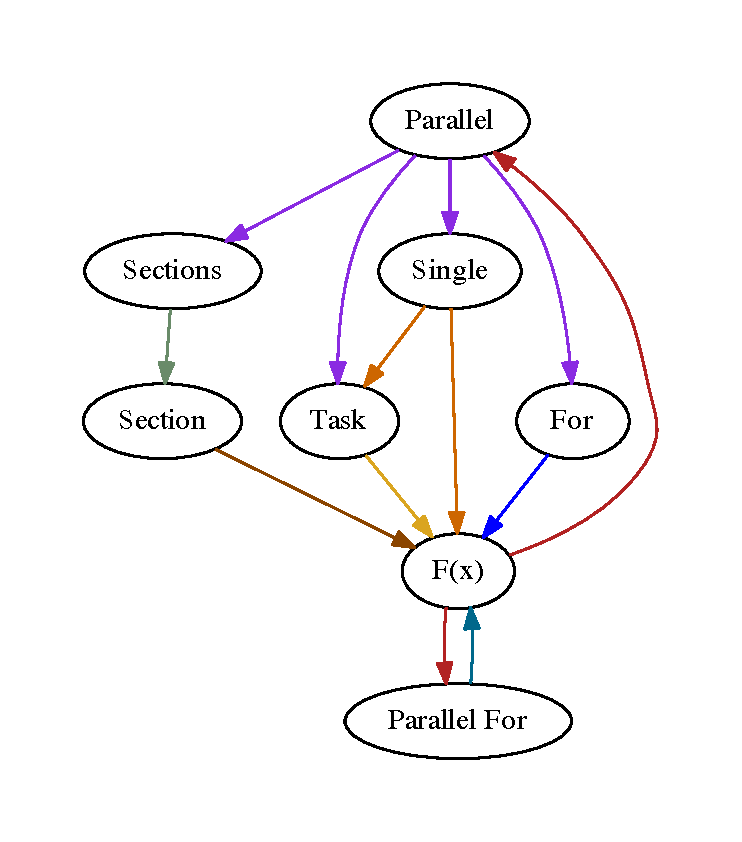
\includegraphics[scale=0.8]{omp.pdf}
\caption{OpenMP directives nested structure.}
\end{figure}

\section{Clang as LLVM frontend}

Clang \cite{clang} is a compiler front-end for the C, C++ and Objective-C programming languages and tit relies on LLVM as back-end. 

A compiler front-end is in charge of analyzing the source code to build the intermediate representation (IR) which is an internal representation of the program. The front-end is usually implemented in three phases: lexing, parsing and semantic analysis. This helps to improve modularity and separation of concern and it allows programmers to use the front-end as a library in their projects. 

The IR is used by the compiler back-end (LLVM in the case of Clang) which transforms it into machine language, operating in three macro phases: analysis, optimization and code generation. 

The LLVM project was started at the University of Illinois at Urbana–Champaign, under the direction of Vikram Adve and Chris Lattner \cite{llvm1} \cite{llvm2}. In 2005 Apple hired Lattner and formed a team to work on the LLVM system for various uses within Apple's development systems; the Clang compiler was born as a project of this team and was open-sourced in 2007. Nowadays its development is completely open-source and besides Apple there are several major software companies involved, such as Google and Intel.

Clang is designed to be highly compatible with GCC and its command line interface is similar to and shares many flags and options with it. Clang was chosen for the development of this framework over GCC for three main reasons:
\begin{itemize}
 \item Clang has proven to be faster and less memory consuming in many situations \cite{clanggcc}. 
 \item Clang has a modular, library based architecture and this structure allows the programmer to easily embed Clang’s functionalities inside its code. Each of the libraries that forms Clang has its specific role and set of functions; in this way the programmer can just simply use the libraries he needs, without having to study the whole system. On the other side GCC's design makes it difficult to decouple the front-end from the rest of the compiler.
 \item Clang provides the possibility to perform code analysis, information extraction and, most important, source-to-source transformation.
\end{itemize}

Clang was not the only alternative to GCC, since also other open-source projects, like the Rose Compiler \cite{rose} and Mercurium \cite{mercurium} were viable options. The Rose Compiler has been developed at the Lawrence Livermore National Laboratory (USA) and it provides the possibility to perform source-to-source transformation and to build code analysis tools, but unfortunately it doesn't support OpenMP. Mercurium has been devolped at the Barcelona Supercomputing Center and it provides source-to-source transformation tools as well as the support to OpenMP, however it has not been chosen because of its little spread, comparing it with Clang. 

The strength of Clang is in its implementation of the Abstract Syntax Tree (AST). Clang’s AST is different from ASTs produced by some other compilers in that it closely resembles both the written C++ code and the C++ standard.

The AST is accessed through the \emph{ASTContext} class. This class contains a reference to the \emph{TranslationUnitDecl} class which is the entry point into the AST (the root) and it also provides the methods to traverse it.

Clang’s AST nodes are modeled on a class hierarchy that does not have a common ancestor; instead, there are multiple larger hierarchies for basic node types. Many of these hierarchies have several layers and branches so that the whole AST is composed by hundreds of classes for a total of more than one hundred thousand lines of code. Basic types derive mainly from three main disjoint classes: \emph{Decl}, \emph{Type} and \emph{Stmt}. 

As the name suggests, the classes that derive from the \emph{Decl} type represent all the nodes matching piece of code containing a declaration of variables (\emph{ValueDecl}, \emph{NamedDecl}, \emph{VarDecl}), functions (\emph{FunctionDecl}), classes (\emph{CXXRecordDec}l) and also function definitions.

Clang’s AST is fully type resolved and this is afforded using the \emph{Type} class which allows to describe all possible types (\emph{PointerType}, \emph{ArrayType}).

Lastly there is the \emph{Stmt} type which refereres to the control flow (\emph{IfStmt}) and loop block of code (\emph{ForStmt}, \emph{WhileStmt}), expressions (\emph{Expr}), return commands (\emph{ReturnStmt}), scopes (\emph{CompoundStmt}), \dots 

Together with the above mentioned three types, there are other “glue” classes that allow to complete the semantic. The most remarkable ones are: the \emph{TemplateArgument} class, that, as the name suggests, allows to handle the template semantic and the \emph{DeclContex} class which is used to extend \emph{Decl} semantic and will be explained later. 

To built the tree the nodes are connected to each other; in particular a node has references to its children. For example a \emph{ForStmt} would have a pointer to the \emph{CompoundStmt} containing its body, as well as to the \emph{Expr} containing the condition and the \emph{Stmt} containing the initialization. A special case is the \emph{Decl} class which is designed not to have children and thus can only be a leaf in the AST. There are cases in which a \emph{Decl} node is needed to have children, like for example a \emph{FunctionDecl} which has to refer to the \emph{CompoundStmt} node containing its body or to the list of its parameters (\emph{ParmVarDecl}). The \emph{DeclContext} class has been designed to solve this issue; when a \emph{Decl} node needs to have children it can just extend the \emph{DeclContext} class and it will be provided with the rights to points to other nodes. 

\begin{figure}[H]
\centering
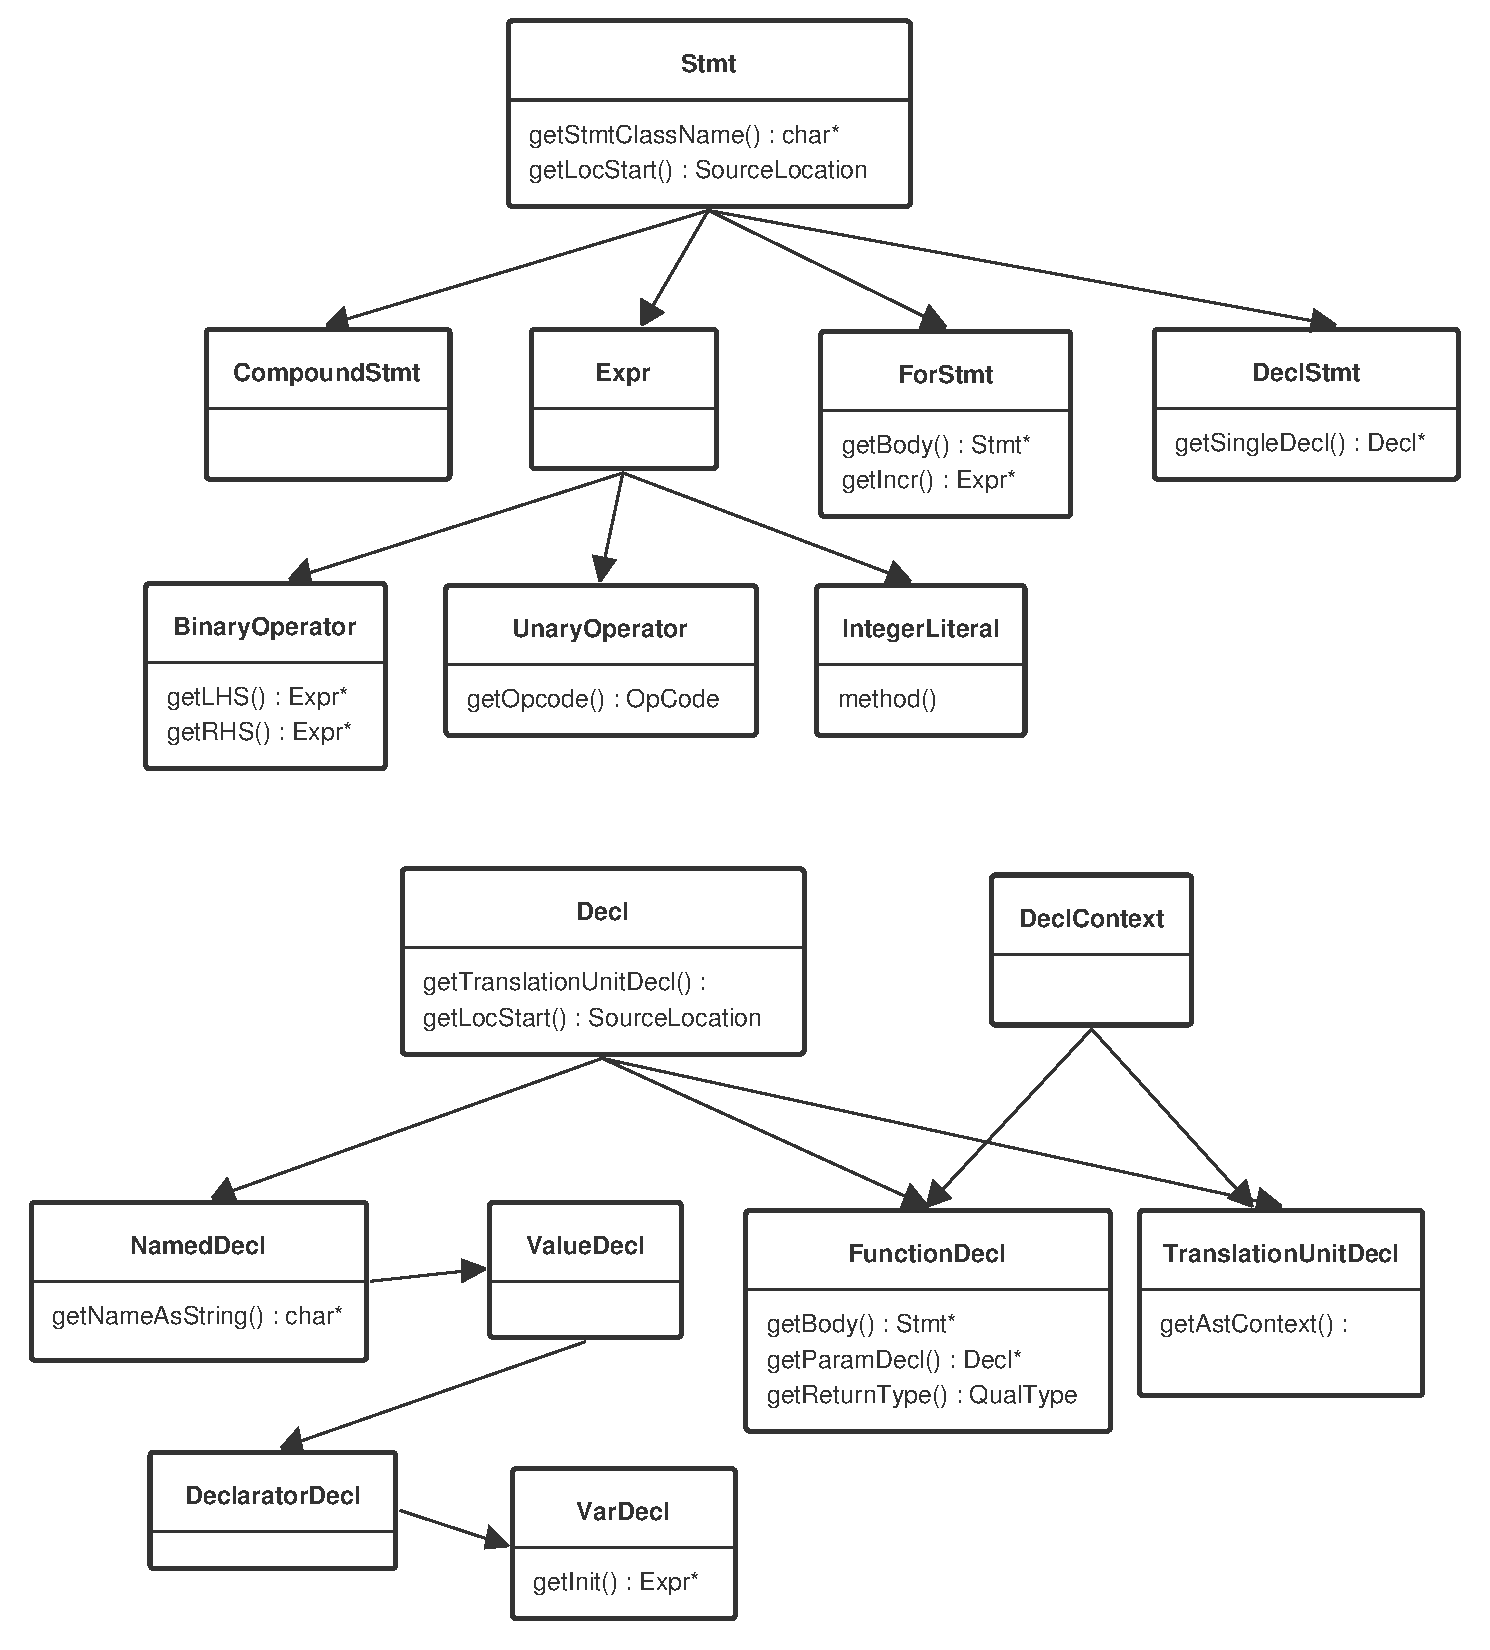
\includegraphics[scale=0.6]{clang_classes.pdf}
\caption{Clang class hierarchy.}
\end{figure}

There are two other classes that are worth mentioning: \emph{SourceLocation} and \emph{SourceManager} class. The \emph{SourceLocation} class allows to map a node to the source code. The \emph{SourceManager} instead provides the methods to calculate the location of each node. These classes are very powerful as they allow to retrieve both the start and the end position of a node in the code, giving the exact line and column number. For example given a \emph{ForStmt}, the \emph{SourceManager} is able to provide the line number of where the stmt starts and ends, but also the column number where the loop variable is declared or where the increment is defined.

To traverse the AST, Clang provides the \emph{RecursiveASTVisitor} class. This is a very powerful and quite easy to learn interface that allows the programmer to visit all the AST’s nodes. The user can customize this interface in such a way that it will trigger only on nodes he is interested in; for example the methods \emph{VisitStmt()} or \emph{VisitFunctionDecl()} are called each time a node of that type is encountered. Each AST node class contains "getter" methods to extract informations out of the code. For example a \emph{Stmt} class has a method to know what kind of \emph{Stmt} the node is, as \emph{IfStmt}, \emph{Expr}, \emph{ForStmt}, \dots. In turn \emph{ForStmt} class provides methods to find the name of the looping variable, the initialization value and the looping condition.

To better understand how the Clang’s AST is structured, Code~\ref{astexemple} and~\ref{ast} contain a simple dummy code and the associated AST.
\newline
\begin{lstlisting}[language=CCC, caption=Simple code., label=astexemple]
class A {
public:
	int x;
	void set_x(int val) {
		x = val * 2;
	}	
	int get_x() {
		return x;
	}
};
int main() {
	A a;
	int  val = 5;
	a.set_x(val);
}
\end{lstlisting}

\begin{lstlisting}[language=AST, caption=Clang AST of the simple code., label=ast]
TranslationUnitDecl
|-CXXRecordDecl <clang_ast_test.cpp:2:1, line:13:1> class A
| |-CXXRecordDecl <line:2:1, col:7> class A
| |-AccessSpecDecl <line:3:1, col:7> public
| |-FieldDecl <line:4:2, col:6> x 'int'
| |-CXXMethodDecl <line:5:2, line:7:2> set_x 'void (int)'
| | |-ParmVarDecl <line:5:13, col:17> val 'int'
| | `-CompoundStmt <col:22, line:7:2>
| |   `-BinaryOperator <line:6:3, col:13> 'int' lvalue '='
| |     |-MemberExpr <col:3> 'int' lvalue ->x
| |     | `-CXXThisExpr <col:3> 'class A *' this
| |     `-BinaryOperator <col:7, col:13> 'int' '*'
| |       |-ImplicitCastExpr <col:7> 'int' <LValueToRValue>
| |       | `-DeclRefExpr <col:7> 'int' lvalue ParmVar 'val' 'int'
| |       `-IntegerLiteral <col:13> 'int' 2
| |-CXXMethodDecl <line:9:2, line:11:2> get_x 'int (void)'
| | `-CompoundStmt <line:9:14, line:11:2>
| |   `-ReturnStmt <line:10:3, col:10>
| |     `-ImplicitCastExpr <col:10> 'int' <LValueToRValue>
| |       `-MemberExpr <col:10> 'int' lvalue ->x
| |         `-CXXThisExpr <col:10> 'class A *' this
| |-CXXConstructorDecl <line:2:7> A 'void (void)' inline
| | `-CompoundStmt <col:7>
| `-CXXConstructorDecl <col:7> A 'void (const class A &)' inline
|   `-ParmVarDecl <col:7> 'const class A &'
`-FunctionDecl <line:15:1, line:21:1> main 'int (void)'
  `-CompoundStmt <line:15:12, line:21:1>
    |-DeclStmt <line:17:2, col:5>
    | `-VarDecl <col:2, col:4> a 'class A'
    |   `-CXXConstructExpr <col:4> 'class A' 'void (void)'
    |-DeclStmt <line:18:2, col:14>
    | `-VarDecl <col:2, col:13> val 'int'
    |   `-IntegerLiteral <col:13> 'int' 5
    `-CXXMemberCallExpr <line:20:2, col:13> 'void'
      |-MemberExpr <col:2, col:4> '<bound member function type>' .set_x
      | `-DeclRefExpr <col:2> 'class A' lvalue Var 'a' 'class A'
      `-ImplicitCastExpr <col:10> 'int' <LValueToRValue>
        `-DeclRefExpr <col:10> 'int' lvalue Var 'val' 'int'
\end{lstlisting}


Clang supports the insertion of custom code through the \emph{Rewriter} class. This class provides several methods that allow, specifying a \emph{SourceLocation}, to insert, delete and replace code and it also allows to replace a \emph{Stmt} object with another one. The programmer cannot know a priori the structure of the input source code, so the best way to insert the custom text, in the correct position, is during the parsing of the AST. It is in fact possible to access each node’s start and end \emph{SourceLocations} reference, to transform them in a line plus column number and insert the text at the end of the line or at line above or below, as needed. 

The text to be rewritten and its position are stored, during the parsing of the AST, in a buffer inside the \emph{Rewriter} object; when the parsing is completed a new source file is generated with the buffer’s data inserted in it.  

Clang’s support to pragmas and OpenMP is really recent. Intel provided an unofficial patched version of the original Clang, which fully supports the OpenMP 3.3 standard, in July 2013 and the patch has not yet been inserted in the official release. Although it is not an official release Intel, has worked inline with the Clang community principle and design strategies and it also produced a complete Doxygen documentation of the code. This patch works jointly with the Intel OpenMP Runtime Library \cite{intelomprtl} which is open-source. 

For what concerns the support to generic pragmas the only remarkable work, that goes close to this goal is the one of Simone Pellegrini. He indeed implemented a tool (Clomp \cite{clomp}) to support OpenMP pragmas in Clang. Clomp is implemented in a modular and layered faschion which this implies that the same structure can be easily used to support customized pragmas.
 



\chapter{Design}
\section{The framework}

The framework takes as input a C++ source code annotated with \emph{OpenMP} and translates each pragma block in a task. After that the tool searches for the best possible schedule which satisfies the tasks timing contrains. The source code is then executed with the given schedule and the help of a newly produced run-time support.

The developed tool works accordingly to the following steps:
\begin{itemize}
\item{the \emph{AST}, Abstract Sintax Tree, of the source code is created using \emph{Clang}. From this all the relevant information of each \emph{OpenMP} pragma are extracted and inserted in a properly formatted \emph{XML} file.}
\item{Each pragma in the source code is substituted with a proper profiling function call. The execution of the new code produces a log file which includes, for each pragma, timing informations.  }
\item{The new source code and the pragma \emph{XML} file are given as imput to a second tool written in \emph{Python}. This tool parses the \emph{XML} file and creates a graph which represents the parallel execution flow of the tasks. After that it executes the given profiled source code $N$ times creating statistics of the execution. The graph, enhanced with the new profiling information, is saved as a new \emph{XML} file}
\item{ A scheduling algorithm is run on the created graph to find the best possible scheduling sequence, accordingly to the profiling information. The found scheduling is then checked to be compatible with the precedence contraints given by the \emph{OpenMP} standard and, in case, a \emph{XML} schedule file is created.}
\item{ The source code is rewritten substituting to each pragma a proper code block for the creation of the tasks. During the execution each task is passed to the run-time support which allocates it accordingly to the previously creted schedule.}
\end{itemize}

Picture \ref{framework} gives a visual representation of the framwork.

\begin{figure}[H]
\centering
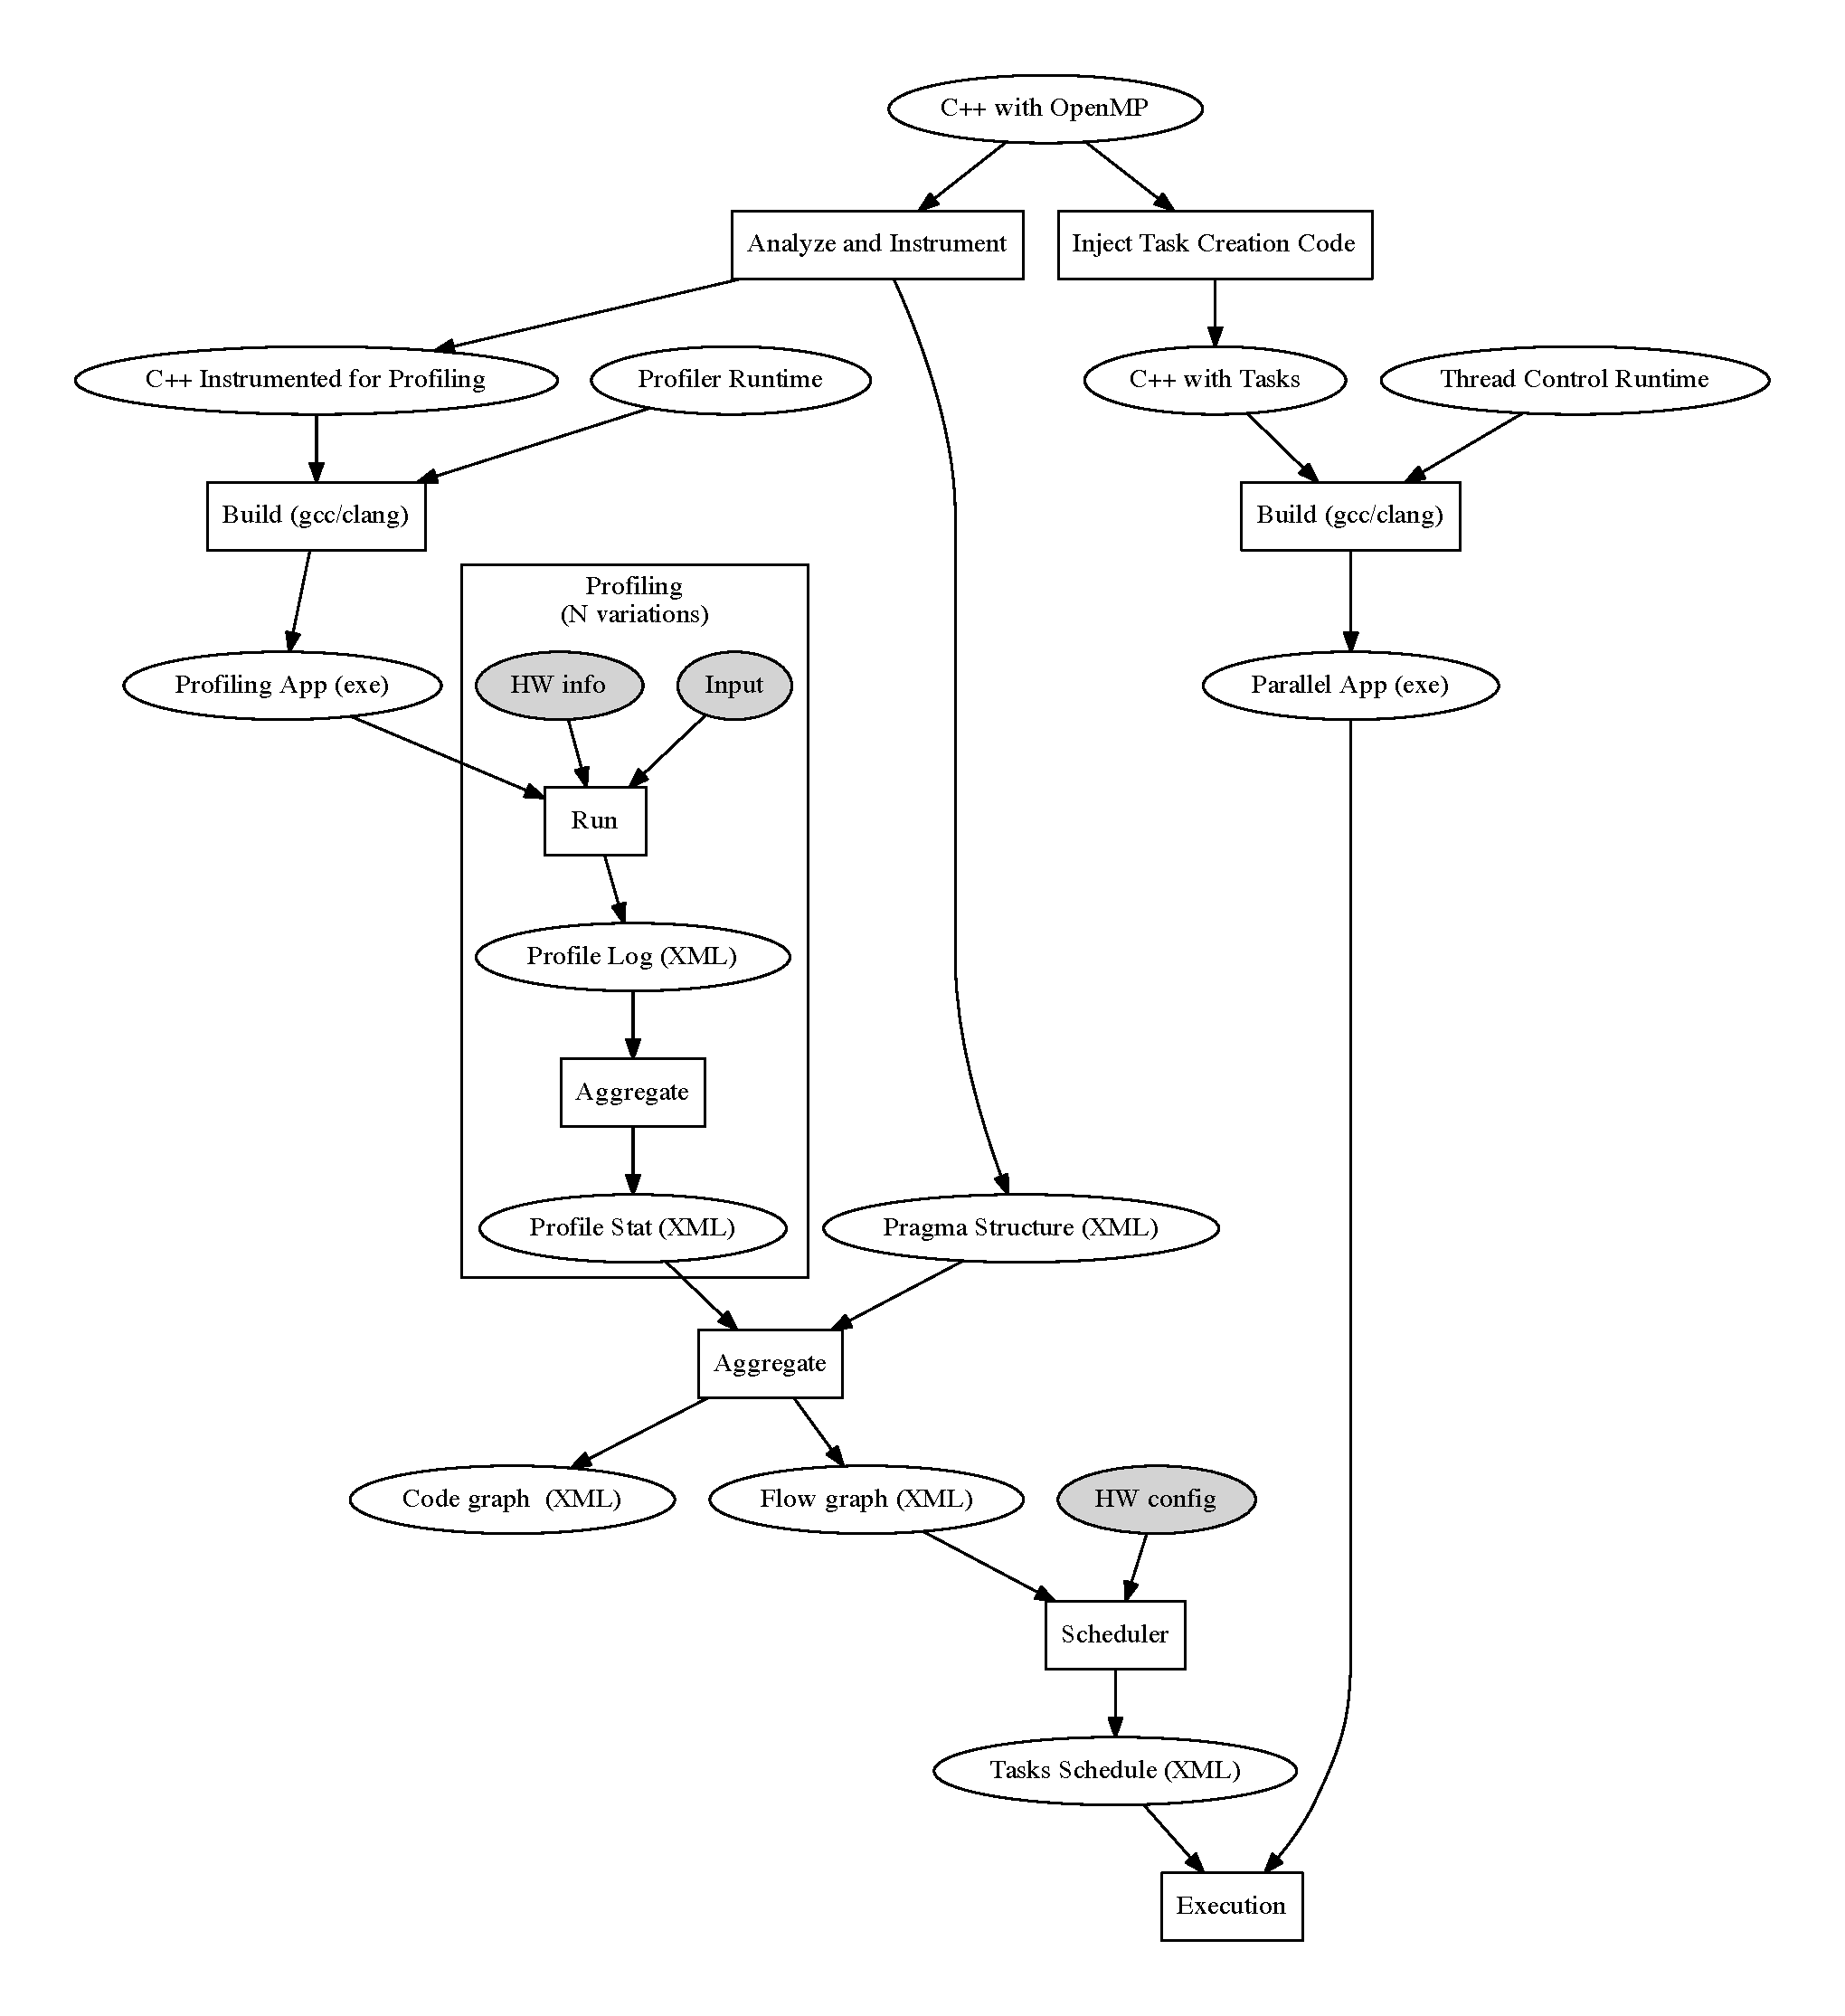
\includegraphics[scale=0.5]{tgraph.pdf}
\caption{The famework structure}
\label{framework}
\end{figure}


\section{A simple example}
\label{example}
A simple example has been developed in order to show how the tool works in each step. Given the \emph{OpenMP} semantic described before, the two \begin{bf}$\#$pragma omp section\end{bf} are executing in parallel and synchronize at the end of the \begin{bf}$\#$pragma omp parallel\end{bf}. The clause \emph{private(bar)} makes the \emph{bar} variable private to each thread in order to have no race condition. To execute the example with some timing constrains some code has been added inside of the for loop which is not relevant for the explaination purpose.

\lstset{language=CCC}
\begin{lstlisting}[caption=Sample code, label=code]
#include <omp.h>

int work(int bar){
    #pragma omp parallel for
    for (int i = 0; i < bar; ++i)
    {
       //do stuff
    }  
    return 0;
};

int main(int argc, char* argv[]) {
    int bar;
    #pragma omp parallel private(bar)
    {
        #pragma omp sections
        {
            #pragma omp section
            {   
                //do stuff (bar)
                work(bar);
            }
            
            #pragma omp section
            {
                //do stuff (bar)
                work(bar);
            }
        }
    }
    return 0;
}

\end{lstlisting}


\section{Analysis}
\subsection{Code}

Chapter presents and justifies the choices that have been made during the parsing of the input source code; in particular which features have been extracted and why.

First of all it will be shown how OpenMP pragmas are translated in the Clang’s AST. The framework targets only a small part of the OpenMP environments, in particular only \emph{parallel}, \emph{sections} (\emph{single}), \emph{section} (\emph{task}) and \emph{for} pragmas. These pragmas have the common property that they are all transformed into \emph{Stmt} nodes in the AST. Each of these pragmas is represented in the AST by a specific class: \emph{OMPParallelDirecetive}, \emph{OMPSectionsDirective} and so on. All these classes inherit from the \emph{OMPExecutableDirective} class which in turn derives from the \emph{Stmt} class. 

These classes have three main functions, one to know the name of the directive associated to it, one to retrieve the list of the clauses and one to get the associated stmt. Based on this last function the above directives can be divided into two groups, the first containing the \emph{for} pragma and the second all the others. The difference between the two groups is that the \emph{for} pragma has associated a \emph{ForStmt}, while the other have associated a \emph{CompoundStmt}. All the clauses derives from a common primitive ancestor which is the \emph{OMPClause} class. 

A real-time program, to be scheduled, needs to provide some informations about its timing constraints, in particular the deadlines; this data can be provided in a separate file or directly inside of the code. In this framework the second approach has been chosen and it has been done using the OpenMP clauses. The standard clauses clearly don’t allow to specify the deadline of a pragma, so a patch has been added to the standard Clang to support the \emph{deadline} clause. This patch can be further enhanced to support other custom clauses, such as the activation time or the period.

The framework parses the source code customizing the \emph{RecursiveASTVisitor} interface; in particular it overrides two methods: \emph{VisitFunctionDecl()} and \emph{VisitStmt()}. Each time the parser comes up with a \emph{FunctionDecl} object or a \emph{Stmt} object it invokes the associated custom function. \emph{VisitFunctionDecl()} adds all objects representing a function definition to a \emph{FIFO} queue.  At the end of the parsing this queue will contain the definition of all the functions in the input source code. \emph{VisitStmt()} instead triggers on each stmt, checking the type and in case of an \emph{OMPExecutableDirective} node it adds it to another \emph{FIFO} queue, that at the end will contain all the pragmas. The two queueus have the property that the order of their elements is given by the positions of the nodes in the source code: the smaller the starting line, the smaller its position in the list. This property is granted by the fact that the input code is parsed top down.

Once all the pragmas are in the queue, the tool inspects each node, extracting information and saving them in a custom class and the newly created objects are used to build a pragma tree. Since an input code can have multiple functions containing OpenMP pragmas and at static time it is not possible to understand where and when these functions will be called, the framework builds different pragma trees, one for each function. It is possible to know, for each function, at which line its body starts and ends and so it is possible to match each pragma to the correct function. The tree structure is given by the nested architecture of the OpenMP pragmas, that has been described in chapter~\ref{openmp}. The building of the tree is quite simple and straightforward as there are several properties that comes handy. The extracted pragmas in the list are ordered according to their starting line, so pragmas belonging to the same function are continuous. Every time a pragma is popped from the list, its starting line is checked and if it belongs to the same function of the previous node it is added to the current tree, otherwise it will be the root of a new tree. Another property is that a pragma is a child of another pragma only if it is nested inside it; to be nested a node must have its starting line greater and its ending line smaller than the other one.  The last property, that still comes from the ordered pragma list and from the definition of nested, is that a node can be nested only in its previous node (in the list) or in the father of the previous node, or in the father of the father and so on.

Algorithm~\ref{tree} represents the pseudocode for the creation of the pragma tree.

\begin{algorithm}[H]
\begin{algorithmic}
%\State \begin{bf}Data\end{bf}: 
\Function{create\_tree}{pragma list L}
\For{pragma \begin{bf}in\end{bf} L }
\State Function f = \Call{get\_function}{pragma}; \Comment{Returns the function where the pragma is defined.}
\State Node n = \Call{create\_node}{pragma, f}; \Comment{Exctract all the information from the AST node and save them in a custom class.}
\If {f is the same function of the pragma exctracted before}
\State Tree.\Call{insert\_node}{n};
\Else
\State Create a new Tree associated with f and set it as the current tree.
\State Tree.root = n;
\EndIf
\EndFor
\EndFunction
\\
\Function{Tree::insert\_node}{Node n}
\State Node last\_node = Tree.last\_node;
\While {last\_node != NULL}
\If {\Call{check\_annidation}{n, last\_node}}
\State last\_node.\Call{add\_child\_node}{n};
\State n.parent\_node = last\_node;
\State \Return
\Else
\State last\_node = last\_node.parent\_node;
\EndIf
\EndWhile
\State Tree.root.\Call{add\_child\_node}{n};
\State n.parent\_node = NULL;
\EndFunction
\end{algorithmic}
\caption{Pseudocode of the algorithm used to create the pragma tree.}
\label{tree}
\end{algorithm}

During the creation of the trees each AST node is transformed in a custom object that will contain only the information useful for the framework: 

\begin{itemize}
\item pragma type: parallel, sections, for, \dots.
\item Start line and end line of the statement associated with the pragma.
\item A reference to the object containing the information of the function where the pragma is defined.
\item A reference to the original AST node.
\item The list of the pragma clauses and of the variables involved. 
\item The list of its children nodes and a reference to its parent node.
\item In case the node is of type \emph{for} or \emph{parallel for} it contains the reference to another object that contains all the information of the For declaration:
\begin{itemize}
\item the name of the looping variable, its type and initial value.
\item The name of the condition variable, or the condition value.
\item The increment.
\end{itemize}
\end{itemize}

The framework supports only the parsing of For statement with the following structure: \newline

$parameter = value \ | \ var$

$c\_op \ = \ < \ | \ > \ | \ <= \ | \ >= $

$i\_op \ = \ ++ \ | \ -- \ | \ += \ | \ -= \ | \ *=$ 

$for([type] \ var \ = \ parameter; \ var \ c\_op \ parameter; \ var \ i\_op \ [parameter])$ \newline


The \emph{ForStmt} class fully supports the C++ For semantic and this means that it would be possible for the framework to support any kind of For declaration. It has been choosen to support only a basic structure because the effort required to expand the semantic it’s very high and, with some slightly modification to the code, it is possible to support almost any possible scenarios. For example a For declaration like this: \\

\begin{lstlisting}[language=CCC]
for (int i = foo(); i < bar*baz; i ++)
\end{lstlisting} 
can be translated as: \\

\begin{lstlisting}[language=CCC]
int init_val = foo();
int cond_val = bar*baz;
for(int i = init_val; i < cond_val; i ++)  
\end{lstlisting}
becoming understandable by the framework.

\begin{figure}
\centering
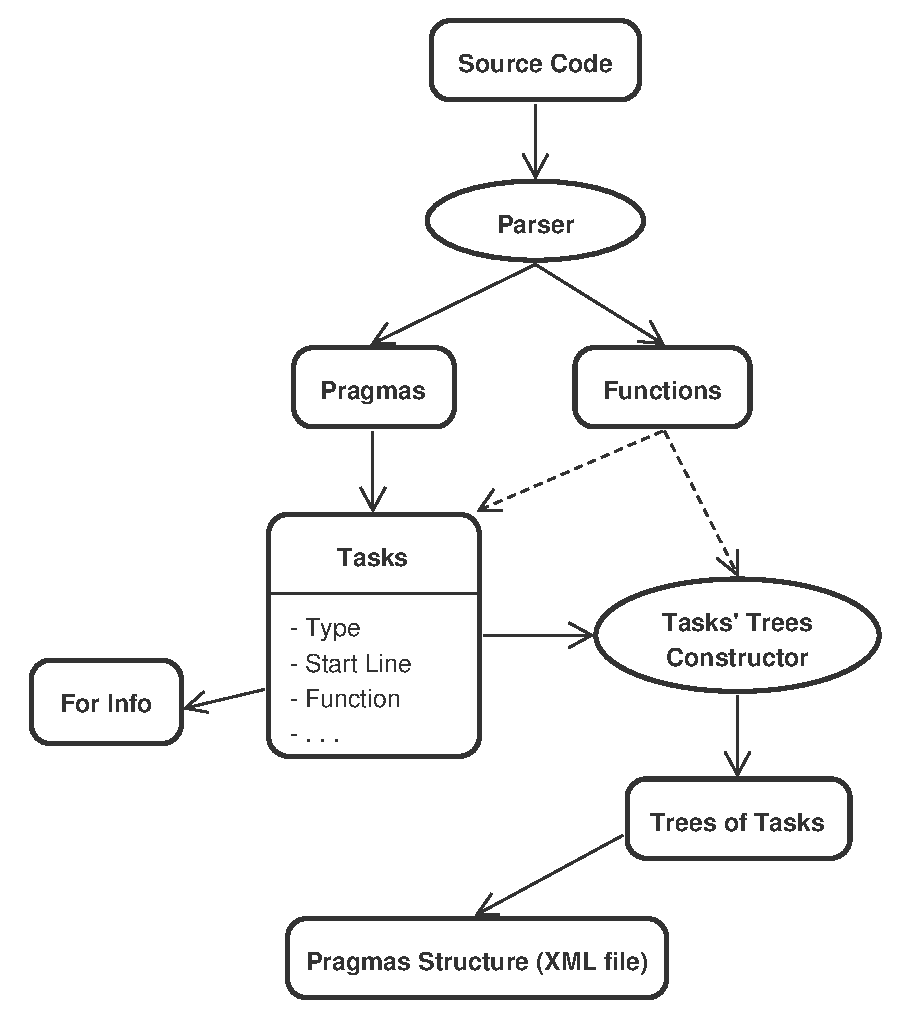
\includegraphics[scale=0.5]{pragma_exctraction.pdf}
\caption{Execution flow of the pragma exctraction.}
\end{figure}

Once all the pragmas have been translated and added in a tree, the new data structures are translated in XML format. Each object is described either by a \emph{Pragma} tag or by a \emph{Function} tag. The two tags contains a list of other tags, one for  each of the variables contained in the tree’s objects. The semantic of XML allows also to translate the original tree structure without loosing informations and this is done by nesting \emph{Pragma} tags one inside the other. The outermost tags are of type \emph{Function}; each function is the root of a tree so it will contain one or more \emph{Pragma} tags. In turn each \emph{Pragma} tag, if containing children nodes in its original tree, will contain other \emph{Pragma} tags. Code~\ref{xmlpragma} represent a portion of the XML code generated from the sample code in paragraph~\ref{example}.

\begin{lstlisting}[language=XML, caption=XML file of the pragma structure of Code~\ref{code}., label=xmlpragma]
<File>
    <Name>omp_test.cpp</Name>    
    ...
    <Function>
        <Name>main</Name>
        <ReturnType>int</ReturnType>
        <Parameters>
            <Parameter>
                <Type>int</Type>
                <Name>argc</Name>
            </Parameter>
            <Parameter>
                <Type>char **</Type>
                <Name>argv</Name>
            </Parameter>
        </Parameters>
        <Line>12</Line>
        <Pragmas>
            <Pragma>
                <Name>OMPParallelDirective</Name>
                <Options>
                    <Option>
                        <Name>private</Name>
                        <Parameter>
                            <Type>int</Type>
                            <Var>bar</Var>
                        </Parameter>
                    </Option>
                </Options>
                <Position>
                    <StartLine>15</StartLine>
                    <EndLine>30</EndLine>
                </Position>
                <Children>
                    <Pragmas>
                        <Pragma>
                            <Name>OMPSectionsDirective</Name>
                            <Position>
                                <StartLine>17</StartLine>
                                <EndLine>29</EndLine>
                            </Position>
                            <Children>
                                <Pragmas>
                                    <Pragma>
                                        <Name>OMPSectionDirective</Name>
                                        <Position>
                                            <StartLine>19</StartLine>
                                            <EndLine>22</EndLine>
                                        </Position>
                                    </Pragma>
				...
</File>
\end{lstlisting}

This XML file will then be passed to the scheduler algorithm, that will add a semantic to each node to build a parallelization graph  which will be then used to create the tasks’ schedule. The original trees are not discarded and they will be used to produce the final code during a following parsing step.

\subsection{Parallelism}
\label{paralelism}

Using the previously created XML file, which contains all the pragmas present in the source code, two different graphs are created. The first one reflects the pragmas structure, while the second one displays the execution flow of the different pragma blocks. Each pragma is represented by a node which contains all the relevant informations. All nodes derive from a general \emph{Node} class; the most relevant attributes are the following:
\begin{itemize}
\item{ptype : represents the type of the pragma.}
\item{start\_line : represents the code line where the pragma block starts.}
\item{children : a list of all the children pragmas.}
\item{parents : a list of all the pragma parents.}
\item{time : the execution time of the pragma.}
\item{variance : the variance of the execution time.}
\item{deadline : the deadline of the task.}
\item{arrival : the arrival time of the task.}
\end{itemize}

Depending on the specific pragma, special classes are derived like \emph{For\_Node} in case of a \begin{bf}\emph{$\#$pragma omp for}\end{bf} or \begin{bf}\emph{$\#$pragma omp parallel for}\end{bf} or \emph{Fx\_Node} in case of a function node.

To create the first graph the tool starts parsing the XML file and creating a proper object for each encountered pragma. It is important to notice that also pragmas which are not actually executed will be inserted in the graphs. 

The second graph is created taking care of the execution semantic given by \emph{OpenMP}. Again the XML file is parsed and an object is created for each pragma. Each object is then connected with the proper ones and if necessary fake \emph{Barrier} nodes are added to guarantee the synchronization given by the standard. This special nodes are added whenever a "control" pragma is encountered; this is due to the fact that this type of pragmas use to have more than one children, creating a sort of diamond topology, which have to synchronize at the end of the pragma block, figure~\ref{call_graph}.

\section{Visual graph generation}

To visualize the code structure, parallel code execution and the function call graph, three different types of graph have been generated, each containing a series of nodes which are connected through undirected edges. The first node of each graph displays the function name along with the total computation time. For each function in the source code a different graph is created in two different formats; for visualization a \emph{PDF} file, while a \emph{DOT} file is created for manipulation purpouses. The code structure graph, simply called \emph{code graph}, shows how pragmas are nested inside each other. Each node displays relevant informations as pragma type, starting line, execution time and variance. The parallel code execution graph, called \emph{flow graph}, shows which nodes can be executed in parallel; some simple rules apply in this case to understand the execution flow:
\begin{itemize}
\item{a node can execute only after all the parents have completed.}
\item{All nodes which have a single parent in common can execute in parallel (this is shown by having the same color for edges which can execute in parallel).}
\item{All nodes have to synchronize on barrier nodes.}
\end{itemize}
In the \emph{call graph} each node invoking a function containing pragmas is connected to the function subgraph by a directed edge, figure~\ref{call_graph}; the execution flow continues after the function call terminates and resumes in the children of the caller node. The semantic of the execution is the same as the one of the \emph{flow graph}.

\begin{figure}[H]
\centering
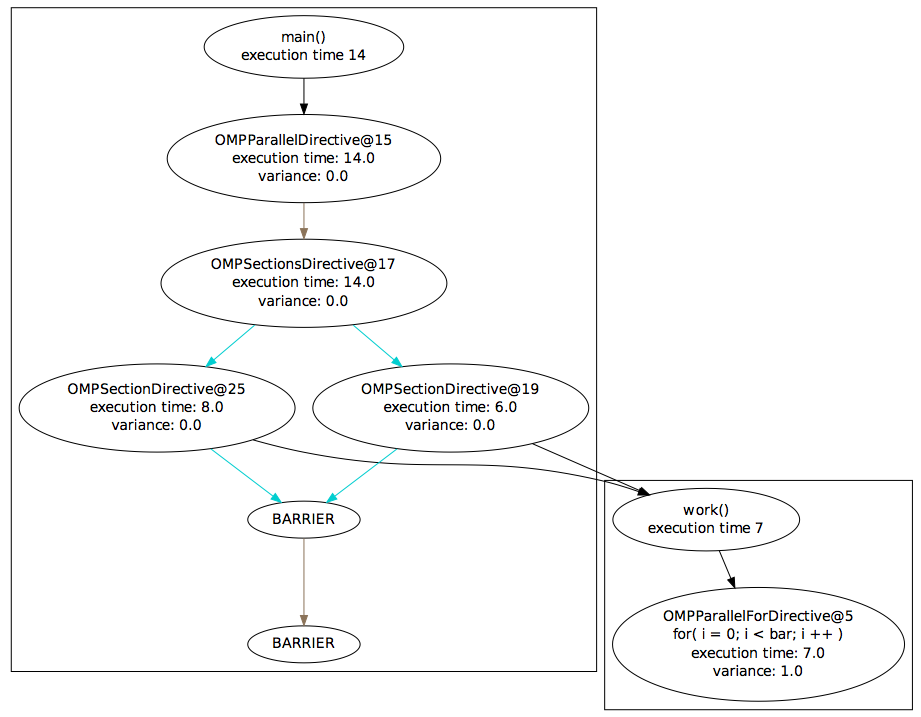
\includegraphics[width = 130mm, height = 76mm]{call_graph.png}
\caption{Call graph example.}
\label{call_graph}
\end{figure}


\section{Intrumentation for profiling}

To produce a good schedule the framework needs informations about the tasks, in particular their computation time, their relations and precedences. Paragraph~\ref{code} shows how pragmas are extracted and their structure; the next step is to retreive the computation time of each task and the functions’ call graph. The only way to get these informations is to profile at run\-time the sequential version of the input code; to have the sequential version, given that the code is parallelized with OpenMP, it is enough to compile it without the \emph{\-fopenmp} flag. 

To be profiled the code needs to be instrumented; in the original code calls to a run-time support are added which calculate the execution time of each tasks, track the caller id of each function and store them in a log file. 

The instrumentation is performed during the first parsing phase of the code, when the pragma statements are collected; the instrumentation does not depend on the semantic of each pragma and makes no distinction between functions and pragmas. The idea is that, each time a pragma or a call to a function is found, a call to the run-time support is inserted. As we have seen in paragraph~\ref{code}, both functions and pragmas have associated either a \emph{CompoundStmt} or a \emph{ForStmt} node. A \emph{CompoundStmt} has the characteristic that it always represents a block of code enveloped in a couple of curly brackets (a scope). In C++ variables declared inside a scope are locally to it, so they are destroyed when the scope ends; the idea is to insert in the original code, at the beginning of the scope, a call to a custom object constructor that starts a timer. When the scope ends the inserted object is destroyed and its destructor is called; the destructor stops the timer and saves the execution time in a log file. 

The tasks can be nested in each other and so the outermost tasks computation time contains the computation time of all its sub-tasks; in other words, the sum of all the tasks’ computation time could exceed the total computation time of the program. To obviate to this problem a method has been designed so that each task can keep track of the computation time of its children in order to obtain its effective computation time. This method allows also to keep track of the caller identity of each pragma and function which is always either another pragma or function.

This method works as follows: there is a global variable that stores the identity of the current pragma or function in execution. Each time a pragma or a function starts its execution the profiler object is allocate and its constructor invoked. The function adds a reference of the pragma/function in the global variable and saves the old value as it identifies its caller. When the object is destroyed the destructor is invoked and it communicates to its caller its computation time, so that the other task can increment the variable containing the children's computation time. Before ending the destructor swaps again the value of the global variable, substituting it with the identifier of its caller. 

In case of a For task the profiler evaluates the number of iterations; this is very important because it helps the scheduler algorithm to decide how much to split the For in the final parallel execution. This evaluation is done subtracting the initial value of looping variable from its ending value and dividing for the increment. This method is not perfect because it may happen that the value of the looping variable or of the conditional variable are changed inside the For body, changing the number of iterations; however the framework’s target applications are real-time programs, so it is very unlikely to find dynamic For blocks. A possible solution to this problem would be to create a new variable, initialized to zero, that it is incremented by one at each iteration and when the For completes its value is caught and stored in the log file. At the end the log file will contain for each task:

\begin{itemize}
\item the total time of the task, from when it was activated since it terminates.
\item The time of all its nested tasks.
\item The identifier of the pragma or function that called the task.
\item In case of For task the number of iterations.
\end{itemize}

Code~\ref{xmllog} shows the log file of the code~\ref{code}.

\begin{lstlisting}[language=XML, caption=XML file of the pragma structure of Code~\ref{code}., label=xmllog]
<LogFile>
	<Hardware NumberofCores="4" MemorySize="2000"/>
	<Pragma fid="3" pid="5" callerid="3" elapsedTime="6" childrenTime="0" loops="6"/>
	<Function fid="3" callerid="19" elapsedTime="6" childrenTime="6"/>
	<Pragma fid="12" pid="19" callerid="17" elapsedTime="6" childrenTime="6"/>
	<Pragma fid="3" pid="5" callerid="3" elapsedTime="8" childrenTime="0" loops="8"/>
	<Function fid="3" callerid="25" elapsedTime="8" childrenTime="8"/>
	<Pragma fid="12" pid="25" callerid="17" elapsedTime="8" childrenTime="8"/>
	<Pragma fid="12" pid="17" callerid="15" elapsedTime="14" childrenTime="14"/>
	<Pragma fid="12" pid="15" callerid="12" elapsedTime="14" childrenTime="14"/>
	<Function fid="12" elapsedTime="14" childrenTime="14"/>
</LogFile>
\end{lstlisting}


\section{Profiling}

The priviously instrumented code is first executed $N$ times, which is given as input parameter, using as arguments the data contained in a specific text file. At each iteration the algorithm produces, for each function and pragma, their execution time and, in case of a $\#$pragma omp for or $\#$pragma omp parallel for, also the number of executed cycles. This data is gathered during the $N$ iterations and then the mean value of the execution time, executed loops and variance for each node is produced and saved in a log file. 
Code~\ref{meanlog} snipped of the log file produce from the Code~\ref{code}:

\lstset{language=XML}
\begin{lstlisting}[caption=Profile XML file, label=meanlog]
<Log_file>
  <Hardware>
    <NumberofCores>4</NumberofCores>
    <MemorySize>2000</MemorySize>
  </Hardware>
  <Function>
    <FunctionLine>3</FunctionLine>
    <Time>7.0</Time>
    <Variance>1.0</Variance>
    <CallerId>[19, 25]</CallerId>
    <ChildrenTime>7.0</ChildrenTime>
  </Function>
...
  <Pragma>
    <FunctionLine>12</FunctionLine>
    <PragmaLine>25</PragmaLine>
    <Time>8.0</Time>
    <Variance>0.0</Variance>
    <Loops>8</Loops>
    <CallerId>['17']</CallerId>
    <ChildrenTime>8.0</ChildrenTime>
  </Pragma>
  <Pragma>
    <FunctionLine>12</FunctionLine>
    <PragmaLine>19</PragmaLine>
    <Time>6.0</Time>
    <Variance>0.0</Variance>
    <Loops>6</Loops>
    <CallerId>['17']</CallerId>
    <ChildrenTime>6.0</ChildrenTime>
  </Pragma>
...
\end{lstlisting}

The new data is added to the \emph{flow graph} previously produced~\ref{xmlpragma}, to be used later in the scheduling algorithm. This graph is then saved as XML file~\ref{flow} by saving nodes and edged separately, giving each a unique identifier. 


\lstset{language=XML}
\begin{lstlisting}[caption=Final XML \emph{flow graph}, label=flow]
<File>
  <Name>source_exctractor/test_cases/thesis_test/omp_test.cpp</Name>
  <GraphType>flow</GraphType>
  <Function id="30">
    <Name>work</Name>
    <ReturnType>int</ReturnType>
    <Parameters>
      <Parameter>
        <Type>int</Type>
        <Name>bar</Name>
      </Parameter>
    </Parameters>
    <Line>3</Line>
    <Time>7.0</Time>
    <Variance>1.0</Variance>
    <Callerids>
      <Callerid>19</Callerid>
      <Callerid>25</Callerid>
    </Callerids>
    <Nodes>
      <Pragma id="58">
        <Name>OMPParallelForDirective</Name>
        <Position>
          <StartLine>5</StartLine>
          <EndLine>8</EndLine>
        </Position>
        <Callerids>
          <Callerid>3</Callerid>
        </Callerids>
        <Time>7.0</Time>
        <Variance>1.0</Variance>
      </Pragma>
    </Nodes>
    <Edges>
      <Edge>
        <Source>30</Source>
        <Dest>58</Dest>
      </Edge>
    </Edges>
  </Function>
\end{lstlisting}


\section{Schedule generation}
\label{schedulegeneration}

The problem of finding the best possible schedule on a multicore architecture is known to be a \emph{NP} hard problem. Given $N$ tasks and $M$ computing cores, the problem consists of creating $K$, possibly lower than $M$, execution flows in order to assign each task to a single flow. Each flow represents a computing core onto which the task should be run. To find a good solution a recursive algorithm has been developed which, by taking advantage of a search tree, figure~\ref{search_tree}, tries to explore all possible solutions, pruning "bad" brenches as soon as possible. Often the algorithm could not finish in a reasonable time due to the big number of possible solutions; to solve this problem a timer has been added to stop the computation after a certain amount of time given as input. \\

\begin{figure}[H]
\centering
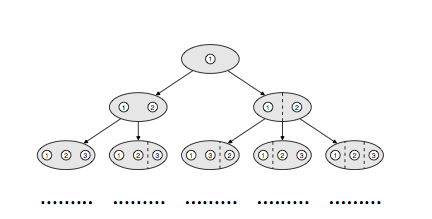
\includegraphics[width = 130mm, height = 76mm]{search_tree.png}
\caption{Search tree.}
\label{search_tree}
\end{figure}

At each level of the search tree a single task is considered; the algorithm inserts the task in each possible flow, checks if the partial solution is feasible and, if affermative, continues until all tasks have been set arriving to a leaf. To check if the partial solution is feasible the algorithm calculates the cost of the actual solution and compares it with the best solution found so far, checks that the number of created flows is less than a predefined number and that the timer has not expired; if all this requirements are met, the brench continues its execution, otherwise it is pruned. After that all tasks are set, if the requirements are fullfilled, the actual solution is compared with the optimal found so far and, in case, the actual one will become the new optimal solution. To calculate if a solution is better than another a simple heuristic has been used: the cost of a task is its computation time, each flow has as cost the summation of all the costs of the containing tasks and the cost of a set of flows (solution or partial solution) is the maximum of the costs of the flows. Given this metric a solution is better than another if it has a lower cost. Having a low flow cost means that the flows are well balanced; it is also important to notice that the algorithm is working in a \emph{breadth-first} manner so that the number of flows is conservative, meaning that the lowest possible number is used to find the best solution. It is possible to easily add any number of pruning and cost metrics to improve the actual search algorithm.

There is a small variation of the algorithm when a task containing a \emph{$\#$pragma parallel for} or \emph{$\#$pragma for} is encountered. In this case the algorithm tryes to split the for loop as much as possible creating new tasks which are added to the task list. First the task is divided in two tasks and they are added to the task list, then the task is splitted in three checking this solution and so on until arriving to the number of available cores. The execution time of each task will be updated accordingly to the number of sub tasks in which it was splitted. 

A parallel version of this algorithm has also been developed in order to check more solutions in the same time. It is important to remember that in Python, even if more threads are created, there is only a single interpreter, so all the threads execution is serialized; to avoid this problem the tool creates different processes, each with its own Python interpreter. Given that the algorithm requires a lot of shared and private data, that is updated at each computation step, the parallelisation of the algorithm would have been extremely complex, so an easier approach has been used. The same sequential algorithm is executed in parallel using for each process a randomized input order of the tasks. In this way each execution will produce all possible solutions in a different order; in any case after a certain amount of time all the processes will find all possible solutions, but with a timing contrain it is very likely that  more solutions are checked. The algorithm terminates returning an optimal solution in the sequantial case and $K$ solutions in the parallel version; in this case the solutions are then compared and the best one is choosen as scheduling sequence.

It is important to notice that such a sequence could in principle not be schedulable, since the algorithm does not take care of precedence relations, but tries only to find the cheapest possible allocation. To check if the solution is feasible a second algorithm has been implemented following a modified version of the the parallel Chetto$\&$Chetto algorithm \cite{bbw2}.

This algorithm works in two phases: the first one sets the deadline for each task, while the second one sets its arrival time. To set the deadlines, the algorithm sets the deadline of all the task with no predecessors to the deadline given in input; after that it recursivly sets the deadline of all tasks wich have all their successors deadline set by calculating the minimum of the difference between the computation time and the deadline of the successor. 

In the second phase the algorithm sets the arrival time of every tasks with no predecessors to zero; after that it recursivly sets the arrival time of all tasks, which have the arrival time of all predecessors set, by calculating the maximum between all the arrival time of the predecessors belonging to the same flow, and the deadline of all the tasks which are assigned to a different flow. This is due to the following fact: let $\tau_j$ be a predecessor of $\tau_i$, written as $\tau_j \rightarrow \tau_i$, with arrival time $a_i$ and let $F_k$ be the flow $\tau_i$ belongs to. If $\tau_j \in F_k$, then the precedence relation is already enforced by the previously assigned deadlines so it is sufficient to ensure that task $\tau_i$ is not activated before $\tau_j$. This can be achived by ensuring that:
\begin{center}$ a_i \ge  {a_i}^{prec} = \smash{\displaystyle\max_{\tau_j \rightarrow \tau_i,\tau_j \in F_k} }\{a_j$\}.\end{center}
If $\tau_j \notin F_k$, we cannot assume that $\tau_j$ will be allocated on the same physical core as $\tau_i$, thus we do not know its precise finishing time. Hence, $\tau_i$ cannot be activated before $\tau_j$'s deadline $d_j$, that is:
\begin{center}$ a_i \ge  {d_i}^{prec} = \smash{\displaystyle\max_{\tau_j \rightarrow \tau_i,\tau_j \notin F_k} }\{d_j$\}.\end{center}
The algorithm checks then that all the deadlines and arrival times are consistent and in case produces the scheduling schema.

\section{Instrumentation for the execution}
\label{designexecution}

This paragraph will present the design strategies that have been used to instrument the input code to make it run accordingly to the schedule produced by the framework. 

The framework needs to be able to isolate each task and execute it in the thread specified by the schedule; to do so new lines of code are added in the original code to transform the old pragmas in a collection of atomic independent concreate tasks. In this phase the functions are not considered as tasks and they won’t be affected by the instrumentation. This is due to the fact that functions have no parallel semantic themselves and they can be simply executed by the tasks that invoke them, without affecting the semantic and improving the efficiency.

The idea of this phase is to transform each pragma block of code into a function which will be called by the designated thread. One possibility is to take the code of the pragma, remove it from the function where it is defined and put it in a newly generated function; this way may be feasible with Clang but it is very complicated because of the presence of nested pragmas. 

The other possibility, used in the framework, is to exploit, once again, the property of the pragmas to be associated with a scope. In C++ it is possible to define a class inside a function if the class is contained in a scope. By exploiting this property each pragma code has been enveloped inside a class declaration; in particular it constitutes the body of a function defined inside the new class.

In the case of a \emph{for} pragma the framework needs to perform some additional modifications of the source code. Usually a For is splitted on more threads in the final execution so the For declaration has to be changed to allow the iterations to be scattered between different threads. Two variables are added to the For declaration: an identifier, to distinguish the different threads and the number of threads concurring in the execution of the For. Here an example:

\begin{lstlisting}[language=CCC]
for(int i = begin; i < end; i ++)
\end{lstlisting}
becomes

\begin{lstlisting}[language=CCC]
int id; //incremental identifier of the task
int num_threads; // number of threads concurring in the execution of the for;
for(int i = begin + id * (end - begin) / num_threads; i < (id + 1) * (end - begin) / num_threads; i ++)
\end{lstlisting}
so if $num\_threads  = 4$, $begin = 0$, $end = 16$, each thread will execute four iterations and in particular the third thread, with $id = 2$ (identifier starts always from zero), will execute:
\begin{lstlisting}[language=CCC]
int new_begin = 0 + 2 *(16 - 0) / 4;
int new_end = 0 + (2 + 1) * (16 - 0) / 4;
for(int i = 8; i < 12; i ++)
\end{lstlisting}

After the definition of the class, at the end of the scope, the framework adds a piece of code that instantiates an object of the created class and passes it to the run-time support. The object will be collected by the designated thread which will invoke the custom function that contains the original code, running it. 

This approach does not change the structure of the code, in particular nested pragmas remain nested; this means that there will be classes definition inside others classes and more precisely there will be tasks inside other tasks. This may seem a problem because it creates dependencies between tasks, not allowing a fully customizable schedule, but this is not true. According to the OpenMP semantics each task is not fully independent from the others and there can be precedences in the execution, but this approach grants that if two tasks can be run in parallel there will be no dependencies between them. To understand this it is necessary to remind the OpenMP structure illustrated in paragraph~\ref{openmp}, where it is explained that two pragmas containing computation code can be related only if in two different functions. 


\section{Run-time support}

This chapter will present how the run-time support for the execution of the final program has been designed. The aim of the run-time is to instantiate and manage the threads and to control the execution of the tasks. In particular it must allocate each task on the correct thread and must grant the precedence constraints between tasks. The run-time must have a very low execution overhead in order to satisfy all the tasks' timing constraints. For this reason the run-time does no time consuming computations and all its allocation decisions are made based on what is written in the schedule. All the heavy calculations, to decide the tasks allocation, has been already done by the schedule algorithm before the program execution and the produced schedule is taken as input by the program. 

Now the execution of the run-time will be presented step by step. First of all the run-time parses the schedule file extracting all the information and storing them in its variables; it then instantiates a threads pool as large as specified in the schedule and creates a job queue for each thread. 

Every time the main program invokes the run-time support it passes to it the object containing the function to be executed. The run-time embeds the received object in an ad-hoc class, that includes the methods and variables needed to perform synchronization on that task. The created job is inserted in a vector shared by all threads; at this point the run-time searches which thread has been designated to run that job and puts an identifier of the job in that thread’s job queue. In case of a For task the run-time has to execute some additional steps: if For task is splitted on more threads the run-time has to duplicate the task for each thread involved; each copy is initialized with an incremental identifier starting from zero and it also receives the total number of threads concurring in the execution of the task. These values are mandatory to inform each thread about the iterations of the For it has to execute. 

Each thread executes an infinite loop; at the beginning of each iteration the thread checks if its queue contains a references to a job and in case pulls the first identifier usesing it to retrieve the real job in the shared vector and executes it. When the job ends the thread checks the schedule to see if it has to wait for other tasks to complete. After that the thread notifies that the job has been completed so that any other thread waiting on that job can continue their executions. The common jobs’ vector is needed because it allows to share information of a task between all the threads, in particular it is fundamental to perform task synchronization. In Code~\ref{code} the \emph{Sections} task at line 16, after launching its children tasks, has to wait for them to complete in order to finish. This rule is true for each “control” pragma that has children. 

\begin{figure}[H]
\centering
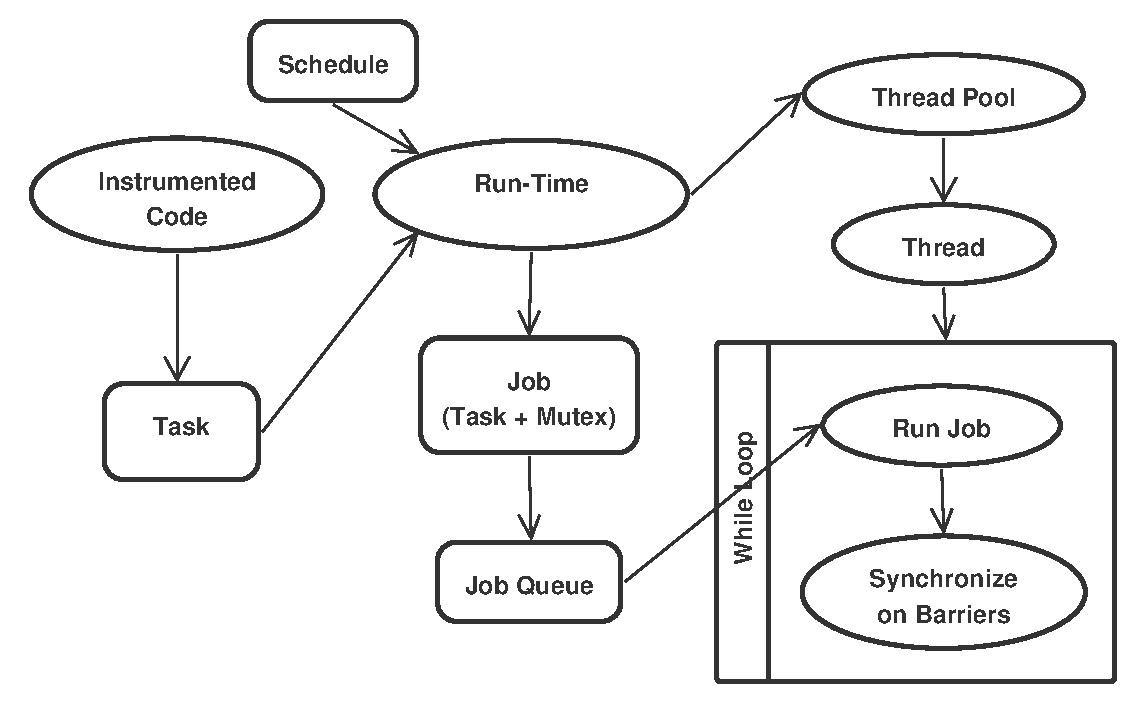
\includegraphics[scale=0.6]{runtime_execution.pdf}
\caption{Flow execution of the runtime support.}
\end{figure}


\chapter{Implementation}
\section{Scheduling XML schema}
\label{schedulexmlschema}

The schedule schema is produced by the scheduling algorithm only if a feasible solution is found; in this case an XML file is produced containing all the relevant informations for each task, which can be either a function node ora a pragma node. Each node contains the following fields:
\begin{itemize}
\item{\emph{id} : represents the starting line of the task; note that this is not a unique identifier.}
\item{\emph{caller\_id} : contains the caller task (pragma or function); the couple (\emph{id}, \emph{caller\_id}) represents a unique identifier.}
\item{\emph{Type} : represents the type of the pragma or the function name. }
\item{\emph{Threads}/\emph{Thread} : contains a list of integer values representing the number of the core on which to schedule the task. The list will contain only one element for all pragmas, except in case of a \emph{$\#$omp parallel for} and \emph{$\#$omp for} which are splitted.}
\item{\emph{Start\_time} : contains the start time calculated by the Chetto\&Chetto algorithm.}
\item{\emph{Deadline} : represents the deadline for the tasks execution.}
\item{\emph{Barrier}/\emph{id} : contains a list of task ids which identifies the tasks that have to synchronize after terminating the execution.}
\end{itemize}
Part of the XML produced for the example \ref{code} is shown  in \ref{schedule}

\lstset{language=XML}
\begin{lstlisting}[caption=Schedule XML, label=schedule]
<Schedule>
  <Cores>4</Cores>
  <Pragma>
    <id>12</id>
    <Caller_id>0</Caller_id>
    <Type>main</Type>
    <Threads>
      <Thread>0</Thread>
    </Threads>
    <Start_time>0</Start_time>
    <Deadline>22.0</Deadline>
    <Barrier>
      <id>15</id>
    </Barrier>
  </Pragma>
  <Pragma>
    <id>15</id>
    <Caller_id>12</Caller_id>
    <Type>OMPParallelDirective</Type>
    <Threads>
      <Thread>0</Thread>
    </Threads>
    <Start_time>0</Start_time>
    <Deadline>22.0</Deadline>
    <Barrier>
      <id>15</id>
      <id>17</id>
    </Barrier>
  </Pragma>
...
<Pragma>
    <id>5</id>
    <Caller_id>3</Caller_id>
    <Type>OMPParallelForDirective</Type>
    <Threads>
      <Thread>2</Thread>
      <Thread>3</Thread>
    </Threads>
    <Start_time>27.0</Start_time>
    <Deadline>30.0</Deadline>
    <Barrier>
      <id>5</id>
    </Barrier>
  </Pragma>
...

\end{lstlisting}

\section{Graph creation}
\label{graph}

After the profiling step, the different types of gaphs described in paragraph~\ref{paralelism} are created. To generate the main graph, the \emph{flow graph}, which represents the execution flow of the program, the following pseudo code has been implemented:

\begin{algorithm}[H]
\begin{algorithmic}
\State \begin{bf}Data\end{bf}: pragma\_xml = list of pragmas, profile\_xml = profile log
\Function{getParalGraph}{ pragma\_xml, profile\_xml}
\State \begin{bf}do\end{bf}: create map with the profile informations
\State \begin{bf}do\end{bf}: g\_list = new list of graphs
\For{f  \begin{bf}in\end{bf} pragma\_xml.functions }
\State g\_list.append(f)  \Comment{create a new graph and add it to graph list}
\State \Call{scan}{f, pragma\_xml} \Comment{starts the creation of the graph}
\EndFor
\State return (g\_list, visual\_g\_list) \Comment{returns the object  and the visual graph}
\EndFunction
\end{algorithmic}
\caption{Pseudocode of the algorithm which produces the object and visual graphs}
\begin{algorithmic}
\Function{scan}{pragma\_xml, profile\_xml, \dots}
\For{p  \begin{bf}in\end{bf} pragma\_xml.pragmas }
\State p.\Call{add\_info}{profile\_xml}
\State add p to the object graph
\State g\_obj = New g\_node(p) \Comment creates a new graphical node
\If {p.children != Null}
\State barrier = \Call{create\_diamond}{pragma\_xml, profile\_xml, p, g\_obj, \dots}
\State p.\Call{add\_barrier}{b}
\EndIf
\EndFor
\EndFunction
\end{algorithmic}

\begin{algorithmic}
\Function{create\_diamond}{pragma\_xml, profile\_xml, p,  g\_obj, \dots}
\For{k  \begin{bf}in\end{bf} p.pragmas }
\State k.\Call{add\_info}{profile\_xml}
\State Add k to the graph
\State g\_obj = New g\_node(k) \Comment creates a new graphical node
\If {k.children != Null}
\State b = \Call{create\_diamond}{pragma\_xml, profile\_xml, k, \dots}
\State k.\Call{add\_barrier}{b}
\Else 
\State b = New barrier
\State k.\Call{add\_barrier}{b}
\EndIf
\EndFor
\State return b
\EndFunction

\end{algorithmic}
\end{algorithm}

\emph{getParalGraph()} creates a list of graphs, one for each function encountered in the pragma XML file created in Code~\ref{xmlpragma}; the \emph{scan()} function is called for each one, in order to create and add all the pragma nodes encountered while reading the XML file. All the informations found in the profile log, created in Code~\ref{meanlog}, will be added to the each pragma node. The \emph{scan()} function has to call a special function, \emph{create\_diamond()}, when a pragma node whith nested nodes is encoutnered; this is due to the fact that special barrier nodes have to be added to maintain the OpenMP synchronization semantic. \emph{create\_diamond()} is a recursive function given that there could be pragma nodes nested inside nested pragma nodes. For each function not only the object graph is created, but also the graphical one using the \emph{pydot} library, a Python interface to the \emph{Graphviz dot} language. To visualize the graphical graphs \emph{Zgrviewer} can be used, a graph visualizer implemented in Java and based upon the \emph{Zoomable Visual Transformation Machine} \cite{zvtm}.


\section{Profiling implementation}
This chapter will show the structure and the implementation of the instrumented code and of the run-time support for the profiling phase.

The first crucial decision that was made was how to identify each pragma and function. There was the necessity to find a method to produce globally unique identifiers which had to be consistent throughout the framework. One possibility was to use some standard identifier generator algorithm; however this approach is not feasible for this framework as it is composed of several cooperative tools and it would have been difficult to keep the identifiers coherent among the different phases. The decision has been made analyzing the characteristic of the environment: first of all the framework operates on one input file at a time and if an input program is composed of multiple files, the tool will produce a different schedule for each. This implies that the identifiers must be unique only for pragmas belonging to the same source file; for this reason the starting line number of each pragma and function has been chosen as the global unique identifier. It is unique because, of course, two pragmas cannot start at the same code line and it is global because it can be retrieved in any part of the framework without having to keep track of it in any data structure throughout the tool execution.

\subsection{Instrumentation}
The instrumentation of the code is composed of two parts: the annotation of the pragmas and the annotation of the functions. These two parts are both performed during the parsing of the AST when a \emph{FunctionDecl} or a \emph{OMPExecutableDirective} is encountered. In the case of a pragma the tool calculates the starting source location of the node which corresponds to the starting line of the associated scope or of the For declaration. The tool adds a comment (\emph{//}) in the line containing the pragma and adds, in the line below,  an If declaration.  This modification to the source code will never break the C++ syntax as the If is always followed either by a scope or by a For declaration. The C++11 standard allows to define variables inside an If declaration so that the lifetime of the new variable is the one of the If block. Code~\ref{profilerif} shows two pieces of the profiling code generated from Code~\ref{code}.

\begin{lstlisting}[language=CCC, caption=Parts of the profiling code generated from Code~\ref{code}., label=profilerif]
...
//#pragma omp parallel for
if( ProfileTracker profile_tracker = ProfileTrackParams(3, 5, bar - 0))
	for (int i = 0; i < bar; ++i)
	{
    		//do stuff
	}
  
...

//#pragma omp section
if( ProfileTracker profile_tracker = ProfileTrackParams(12, 25))
{
    //do stuff (bar)
    work(bar);
}
...
\end{lstlisting}

The structure of the \emph{ProfileTracker} class will be shown later in this paragraph. The code line number of the associated pragma, the container function and, in case of a For declaration, the number of iterations are passed to the constructor of the profiler class.

Code~\ref{functionprofile} shows an example of how functions are annotated for the profiling. 

\begin{lstlisting}[language=CCC, caption=Example of a profiled function from Code~\ref{code}., label=functionprofile ]
...
int work(int bar){
	if( ProfileTracker x = ProfileTrackParams(3, 0)) {
	...
	}
}
\end{lstlisting}

Code~\ref{functionprofile} shows that the structure for profiling functions is almost identical to the one for pragmas; the only difference is that the first parameter of \emph{ProfileTrackParams} matches the line number of the function and the second is always zero. What really changes is how the If is inserted in the code because in this case few additional steps are required as a new scope has to be added. In the first step the If declaration is inserted in the line below of the function’s opening curly bracket, so there is the need to check if the bracket is in the same line of the function or in the underlying line. Second a closing curly bracket must be added at the end of the function definition to close the If scope.

\subsection{Run-time}
\label{profilerun}

This paragraph describes the structure of the two run-time classes involved in the execution of the profiled code. One was already shown in the previous paragraph and the other is \emph{ProfileTrackerLog}. 

\emph{ProfileTrack}’s constructor, when invoked, starts the timer for the current block, invokes \emph{ReplaceCurrentPragma(this)} which updates \emph{ProfileTracker *current\_pragma\_executing\_} with the input value and returns the old value of the variable. The returned value is saved in \emph{previous\_pragma\_executed\_} and identifies the caller id of the current pragma or function. \emph{current\_pragma\_executing\_} holds the reference to the pragma or function that is currently executing, it is used to track the caller id of each block and to create the call graph. 

When the If completes, the \emph{ProfileTrack} object is destroyed and its destructor invoked. The destructor stops the timer and calculates the elapsed time of the block adding it to the children time of its caller block and it writes all the data in the log file, as shown in Code~\ref{xmllog}. At the end, the destructor, calls again \emph{ReplaceCurrentPragma()} passing to it \emph{previous\_pragma\_executing\_} and discarding the returned value.

\emph{ProfileTrackerLog} is in charge of managing the log file, opening and closing it and providing the methods to access it. This class must be instantiated the first time a block is encountered and it must be accessible by all the profiler objects. One possibility is to instantiate it at the beginning of the \emph{main()}, but this is not feasible since there is the possibility that the input file does not contain the main and because profiling objects, allocated in other functions, have no chance to get the reference to the \emph{ProfileTrackerLog} object. The second problem could be solved by rewriting each function in the source file adding to their declaration, as a parameter, a reference to \emph{ProfileTrackerLog}. This method was not chosen given that it is more complex than making \emph{ProfileTrackerLog} a singleton class. This solution has many advantages: the first method that accesses the class automatically instantiates it and a singleton class is global, so there is no need to pass its reference to each profiling object. When the program ends, each allocated object is destroyed and its destructor called. \emph{ProfileTrackerLog}'s destructor simply adds the closing tag (\emph{$<$/LogFile$>$}) in the log file and closes it.


\section{Profiling execution}

To create the profiling log, containing all the statistics on the execution, the following pseudo-code has been implemented in Python:

\begin{algorithm}[H]
\begin{algorithmic}
 \State \begin{bf}Data\end{bf}:{ N = number of interations}
\State \begin{bf}do\end{bf}: Create map for containing the execution data
\For{i  \begin{bf}in\end{bf} N }
\State launch executable and create log\_file
\For{pragma  \begin{bf}in\end{bf} log\_file }
\State insert data in map
\EndFor
\For{function  \begin{bf}in\end{bf} log\_file }
\State insert data in map
\EndFor
\EndFor
\State calculate statistics using map\;
\For{value  \begin{bf}in\end{bf} map }
\State write to XML profile\_log
\EndFor
\State return profile\_log
\end{algorithmic}
\caption{Pseudocode of the algorithm which produces the mean profiling log file}
\end{algorithm}

The algorithm starts by reading from input the number of iteration to execute, $N$; after that it launces the executable $N$ times using as arguments the data contained in a \emph{parameter.txt} file. After each execution, the algorithm, reads the produced log\_file and inserts the pragma/function data in a hash table, summing the execution times. After that the $N$ executions statistics are calculated, using the \emph{Numpy} Python package, and inserted in the hash table. The contained data is then used to construct a XML tree using the \emph{cElementTree} module. The so created XML tree is saved as a new profile log called \emph{`executable\_name'\_profile.xml}. The structure of such file is represented in Code~\ref{meanlog} and the last step consists in inserting the statistics in the \emph{flow graph} produced in paragraph~\ref{graph}.


\section{Schedule generating tool}

As described in paragraph~\ref{schedulegeneration}, two versions of the scheduling algorithm have been developed: a sequential version and a parallel version. The main difference between this two algorithms consists in how the results are returned to the caller function. This is due to the fact that in Python, even if more threads are created, there is only a single interpreter, so all the threads execution is serialized; to avoid this problem the tool creates different processes, each with its own Python interpreter. In the sequential version, since the algorithm is working on shared memory, an empty result container can passed directly by the caller to the function which can then modify it. The parallel version uses instead queues implemented in the Python multiprocessing module which provide an easy API to communicate between procesess, based on send and recive operations. 

\begin{algorithm}
\begin{algorithmic}
\Function{get\_optimal\_flow\_single}{flow\_list, task\_list, level, optimal\_flow, NUM\_TASKS, MAX\_FLOWS, execution\_time}
\If {time.clock() $<$ execution\_time}
\State curopt = get\_cost(optimal\_flow)
\State cur = get\_cost(flow\_list)
\If {len(flow\_list) $<$ MAX\_FLOWS and len(task\_list) != level and cur $\leq$ curopt}
\State task\_i = task\_list[level]
\For{flow in flow\_list}
\State flow.add\_task(task\_i)
\State \Call{get\_optimal\_flow\_single}{\dots, level + 1, \dots}
\State flow.remove\_task(task\_i)
\EndFor
\State new\_flow = new Flow()
\State new\_flow.add\_task(task\_i)
\State flow\_list.append(new\_flow)
\State \Call{get\_optimal\_flow\_single}{\dots, level + 1, \dots}
\State flow\_list.remove(new\_flow)
\If{ task\_i is of type 'For'}
\For{i $\in$ MAX\_FLOWS}
\For{j $\in$ i}
\State task = new For\_Node(task\_i)
\State task\_list.append(task)
\EndFor
\State \Call{get\_optimal\_flow\_single}{\dots, level + 1, \dots, NUM\_TASKS + i - 1, \dots}
\EndFor
\EndIf
\Else
\If{len(task\_list) == level and len(flow\_list) $\leq$ MAX\_FLOWS and cur $\leq$ curopt}
\State update optimal\_flow
\EndIf
\EndIf
\EndIf
\EndFunction
\end{algorithmic}
\caption{Pseudocode of the sequential algorithm which produces the schedule }
\end{algorithm}
\begin{algorithm}[H]
\begin{algorithmic}
\Function{get\_optimal\_flow}{flow\_list, task\_list, level, optimal\_flow, NUM\_TASKS, MAX\_FLOWS, execution\_time, queue}
\If {time.clock() $<$ execution\_time}
\State curopt = get\_cost(optimal\_flow)
\State cur = get\_cost(flow\_list)
\If {len(flow\_list) $<$ MAX\_FLOWS and len(task\_list) != level and cur $\leq$ curopt}
\State task\_i = task\_list[level]
\For{flow in flow\_list}
\State flow.add\_task(task\_i)
\State \Call{get\_optimal\_flow}{\dots, level + 1, \dots}
\State flow.remove\_task(task\_i)
\EndFor
\State new\_flow = new Flow()
\State new\_flow.add\_task(task\_i)
\State flow\_list.append(new\_flow)
\State \Call{get\_optimal\_flow\_single}{\dots, level + 1, \dots}
\State flow\_list.remove(new\_flow)
\If{ task\_i is of type 'For'}
\For{i $\in$ MAX\_FLOWS}
\For{j $\in$ i}
\State task = new For\_Node(task\_i)
\State task\_list.append(task)
\EndFor
\State \Call{get\_optimal\_flow}{\dots, level + 1, \dots, NUM\_TASKS + i - 1, \dots}
\EndFor
\EndIf
\Else
\If{len(task\_list) == level and len(flow\_list) $\leq$ MAX\_FLOWS and cur $\leq$ curopt}
\State empty queue
\State update optimal\_flow
\State queue.add(optimal\_flow)
\EndIf
\EndIf
\EndIf
\EndFunction

\end{algorithmic}
\caption{Pseudocode of the parallel algorithm which produces the schedule }
\end{algorithm}

When the main program wants to call the parallel scheduler, it creates for each process to be instantiated the following data:
\begin{itemize}
\item {a task input sequence by randomizing the task\_list.}
\item{An empty solution container.}
\item{A multiprocessing queue, to return the result from the scheduler process.}
\end{itemize}

After that it creates a new process passing to it a reference to the parallel scheduler function call along with the necessary arguments. All the procesess are then started and the main program remains in a wait state attending the result from the shared queues; after receiving the results, all the processes are joined and the best solution of all the executions is chosen.

As described in paragraph~\ref{schedulegeneration} it is possible that the scheduler splits pragma \emph{for} and pragma \emph{parallel for} onto different threads. In this case new tasks are created which have to be added to the \emph{flow graph} created in paragraph~\ref{graph}. To do so all the new nodes are inserted in a hash table along with all the necessary informations of the originating node; after that the \emph{add\_new\_tasks(\dots)} function is invoked which taskes care of finding, for each new node, the originating node and substituting to it all the new splitted nodes. It is also necessary to add to all nodes the identifing flow id which has been calculated before by the scheduling algorithm.

After creting the new final \emph{flow graph} and the schedule, it is necessary to check if the last one is feasible using the modified version of the Chetto\&Chetto algorithm.

\begin{algorithm}[H]
\begin{algorithmic}
\Function{chetto}{flow\_graph, deadline, optimal\_flow}
\State node = get\_last(flow\_graph)
\State node.deadline = deadline
\State \Call{chetto\_deadlines}{node}
\State node = get\_first(flow\_graph)
\State \Call{chetto\_arrival}{node, optimal\_flow}
\EndFunction

\end{algorithmic}

\begin{algorithmic}
\Function{chetto\_deadlines}{node}
\If{node.parent != Null}
\For{p $\in$ node.parent}
\State p.deadline = \Call{get\_min}{p} 
\EndFor
\For{p $\in$ node.parent}
\State \Call{chetto\_deadlines}{p}
\EndFor
\EndIf
\EndFunction

\end{algorithmic}

\begin{algorithmic}
\Function{chetto\_arrival}{node}
\If{node.children != Null}
\For{child $\in$ node.children}
\If{child.arrival == Null and \Call{all\_set}{child} == True } 
\State (a,d) = \Call{get\_max}{child, optimal\_flow} 
\State child.arrival = max(a,d)
\EndIf
\State \Call{chetto\_arrival}{child, optimal\_flow}
\EndFor
\EndIf
\EndFunction

\end{algorithmic}
\caption{Pseudocode of the modified Chetto\&Chetto algorithm }
\end{algorithm}

The \emph{get\_min()} function just returns the minium deadline which has been set among all the children of a node. The \emph{get\_max()} function returns the maximum deadline and arrival time found based on the criterions described in chap \ref{schedulegeneration}. \emph{all\_set()} checks if all arrival times are set in the parents of a node.

After the \emph{chetto} call, the main program checks if all the deadlines and arrival times are positive and in case constructs the scheduling graph taking care of adding all the necessary synchronization barriers; the schedule is shown in Code~\ref{schedule}. The barriers are added accordingly to the following rules:
\begin{itemize}
\item {every task must be present in at least one barrier tag, meaning that some other task has to wait for the termination of its execution.}
\item {The pragma \emph{parallel} has itself and all its children in the barrier section. (It has not its grandchildren)}
\item {The pragma \emph{parallel for} has only itself as barrier, since its execution will be synchronized directly by the run-time support.}
\item {All the other pragmas have to synchronize on all, and only, their children.}

\end{itemize}

\section{Final Execution}
\subsection{Instrumentation}
This paragraph will describe in details how the code is actually transformed accordingly to what was described in paragraph~\ref{designexecution}.

This phase deals only with pragmas and does not treat functions; if a pragma calls a function it will be considered as part of the pragma and it will be execute on the same thread. Of course if this function contains pragmas, these will be transformed in tasks and allocated as stated in the schedule.

Code~\ref{simpleinstrumentation} shows how the pragma \emph{section} at line 19 of Code~\ref{code} has been transformed into a task.

\begin{lstlisting}[language=CCC, caption=Example of an instrumented \emph{section} pragma from Code~\ref{code}., label=simpleinstrumentation]
 //#pragma omp section
{
    class Nested : public NestedBase {
    public: 
        virtual shared_ptr<NestedBase> clone() const { 
          return make_shared<Nested>(*this); 
        } 
        Nested(int pragma_id, int & bar) : 
            NestedBase(pragma_id), bar_(bar) {}
        int & bar_;
            
        void fx(int & bar){   
            //do stuff (bar)
            work(bar);
            launch_todo_job(); 
        }
        void callme() {
            fx(bar_);
        }
    };
    shared_ptr<NestedBase> nested_b = make_shared<Nested>(19, bar);                             
    if(ThreadPool::getInstance()->call(nested_b)) 
        todo_job_.push(nested_b); 
}
\end{lstlisting}

All the pragma’s code is wrapped in the \emph{fx()} function which belongs to the \emph{Nested} class, that is defined inside the pragma’s scope. The class \emph{Nested} has as parameter \emph{bar\_} which is the variable used inside the pragma block; in general each variable, of any kind, that is used inside the pragma block, but declared outside, is transformed into a class's variable. This is fundamental because when the object will be delivered to the designated thread, it will have a different scope. All the variables used inside a pragma node are stored in the AST and so it is quite easy to retrieve them. The \emph{OMPExecutableDirective} has the reference to an associated statement of type \emph{CapturedStmt} which has the reference to the \emph{CompoundStmt} or \emph{ForStmt} containing the code of the pragma and a reference to the list of all the \emph{VarDecl} objects representing variables used in it. The \emph{clone()} function is necessary for the instrumentation of \emph{for} pragmas and will be described later.

What happens when Code~\ref{simpleinstrumentation} is executed? When the program enters the scope it jumps the class declaration and goes straight to line 23. Here the \emph{Nested} object, corresponding to the pragma \emph{section}, is instantiated: its constructor receives the pragma’s line number and all the parameters that are used inside the code, specifically in this case only the variable \emph{bar}. The constructor initializes its parameters which will be later used by \emph{fx} and calls the costructor of its super class (\emph{NestedBase}) passing to it the pragma identifier.  \emph{NestedBase} is a virtual class declared inside the run-time support which is anchestor of all the classes declared inside the instrumented code and it will be described in the following paragraph. Once the \emph{nested\_b} object is created it is passed to the run-time in the following line. There are other two lines of code that have not been explained: \emph{launch\_todo\_job()} and \emph{todo\_job\_.push(nested\_b)}. These two function calls are necessary to avoid problems during the execution of nested tasks and will be explained in paragraph~\ref{runtime}.

Code~\ref{simpleinstrumentation} shows how \emph{section} pragmas are instrumented; this method is also valid for \emph{task}, \emph{sections}, \emph{parallel}, \dots pragmas, but it is not correct for the \emph{for} pragma. Code~\ref{for} shows how \emph{for} pragmas are instrumented.

\begin{lstlisting}[language=CCC, caption=Example of an instrumented \emph{for} pragma from Code~\ref{code}., label=for]
{
  class Nested : public NestedBase {
  public: 
    virtual shared_ptr<NestedBase> clone() const { 
      return make_shared<Nested>(*this);
    } 
    Nested(int pragma_id, int & bar) : 
        NestedBase(pragma_id), bar_(bar) {}
    int & bar_;

    void fx(ForParameter for_param, int & bar) {
      for(int i = 0 + for_param.thread_id_*(bar - 0)/for_param.num_threads_; 
          i < 0 + (for_param.thread_id_ + 1)*(bar - 0)/for_param.num_threads_; 
          i ++ )
      {
        //do stuff
      }  
      launch_todo_job(); 
    }
    void callme(ForParameter for_param) {
      fx(for_param, bar_);
    }
  };
  shared_ptr<NestedBase> nested_b = make_shared<Nested>(5, bar);
  if(ThreadPool::getInstance()->call(nested_b)) 
    nested_b->callme(ForParameter(0,1));
}
\end{lstlisting}

In case of a \emph{for} pragma the instrumentation becomes a little bit more tricky, but what was true for Code~\ref{simpleinstrumentation} still holds. First of all it is possible to notice that the For declaration has been changed accordingly to what stated in paragraph~\ref{designexecution} and that function \emph{fx()} receives an additional parameter \emph{ForParameter for\_param}. The new parameter is created, passed to the function directly by the run-time and used to specify to each thread which iterations of the For to execute. The \emph{clone()} function, as the name suggests, is used to create copies of the \emph{Nested} object; this is necessary because, when a For is split among different threads, each one needs the object. Threads can’t share the same object since it is most likely that they will execute concurrently, invoking the same function from the same object, creating a race condition. 

The structure of the pragmas in the original source code is not modified during the instrumentation, as explained in paragraph~\ref{designexecution} and this implies that nested pragmas are translated into nested tasks. The consequence of this fact is simply that the outermost tasks, of type \emph{parallel}, are instantiated by the main thread, while the others are allocated and passed to the run-time by the containing task. The overhead to allocate the \emph{Nested} object and to pass it to the run-time is very small, but in any case this approach allows to split this overhead among the threads improving the overall performance. Code~\ref{annidation} shows a piece of the code generated instrumenting Code~\ref{code} illustrating the nested structure of the tasks.

\begin{lstlisting}[language=CCC, caption=Example of tasks annidation from Code~\ref{code}., label=annidation]
int main(int argc, char* argv[]) {
  int bar;
  //#pragma omp parallel private(bar)
  {
    class Nested : public NestedBase {
    public: 
      virtual shared_ptr<NestedBase> clone() const { 
        return make_shared<Nested>(*this); 
      } 
      Nested(int pragma_id, int bar) : 
          NestedBase(pragma_id), bar_(bar) {}
      int bar_;
  
      void fx(ForParameter for_param, int bar){
        //#pragma omp sections
        {
          class Nested : public NestedBase {
          public: 
            virtual shared_ptr<NestedBase> clone() const { 
              return make_shared<Nested>(*this); 
            } 
            Nested(int pragma_id, int & bar) : 
                NestedBase(pragma_id), bar_(bar) {}
            int & bar_;
            
            void fx(ForParameter for_param, int & bar){
              //#pragma omp section
              {
                class Nested : public NestedBase {
  ...
  ...
\end{lstlisting}

\begin{comment}
To complete this paragraph there is only to explain how \emph{barrier} pragmas are annotated; an instrumented \emph{barrier} is shown in Code~\ref{barrier}.

\begin{lstlisting}[language=CCC, caption=Example of \emph{barrier} instrumentation., label=barrier]
{
    class Nested : public NestedBase {
    public:
        virtual shared_ptr<NestedBase> clone() const { 
          return make_shared<Nested>(*this); 
        } 
        Nested(int pragma_id) : NestedBase(pragma_id) {}
        void callme(){}
    };
    ThreadPool::getInstance()->call(make_shared<Nested>(pragma_line));
}
\end{lstlisting}

In OpenMP a \emph{barrier} pragma is used to notifies the run-time that some threads need to synchronize on some tasks and it doesn’t execute any code, so the function \emph{callme()} is simply empty and there is no need for \emph{fx()}. During the execution of the final instrumented code, when the \emph{barrier} is encountered the program instantiate the \emph{Nested} object, passing to it the line number of the pragma and then it passes the object to the run-time. The run-time, when receives the object, consults the schedule, it discovers that it is of type \emph{barrier} and insert, where needed, synchronization points. 
\end{comment}


\subsection{Run-time support}
\label{runtime}
The run-time support for the final parallel execution is composed of two classes: \emph{NestedBase} and \emph{ThreadPool}. \emph{NestedBase} is the virtual class from which every \emph{Nested} class derives; it just stores the identifier (line number) of the corresponding pragma, \emph{int pragma\_id\_}, and a list of tasks, \emph{queue$<$shared\_ptr$<$NestedBase$>>$ todo\_job\_}. This common interface is necessary to handle each task because each \emph{Nested} class, corresponding to a task, exists only inside its scope and it is not usable outside.   

\emph{ThreadPool} is the class that implements the real-time support and it declares two structures: \emph{ScheduleOptions} and \emph{JobIn}. \emph{ThreadPool} has been implemented as a singleton class; the reasons which motivated this choice are the same as the ones shown in paragraph~\ref{profilerun}, for the \emph{ProfileTrackerLog} class. There is no need to protect the instantiation of the class with mutexes given that it is the constructor of this class that instantiates the threads pool.

\emph{ThreadPool}’s constructor parses the input XML schedule file exctracting all the relevant informations. The first tag of the file contains the number of threads to be instantiated; this number is passed to the \emph{init()} function which creates a thread object and pushes it into the thread queue.

\begin{lstlisting}[language=CCC, caption=Initialization of the thread pool., label=pool]
vector<thread> threads_pool_;

threads_pool_.reserve(pool_size);
for(int i = 0; i < pool_size; i++) {
    threads_pool_.push_back(thread(&ThreadPool::run,this, i));
}
\end{lstlisting}

The constructor then parses each \emph{$<$Pragma$>$} block saving the retrieved information inside an object of type \emph{ScheduleOptions} that is inserted in \emph{map$<$int, ScheduleOptions$>$ sched\_opt\_}. The C++ \emph{map$<>$} is implemented as a binary tree, so the cost for retrieving the schedule options of a given pragma is $\mathcal{O}(log(n))$, where $n$ is the number of pragmas.  Code~\ref{schedopt} shows the structure of \emph{ScheduleOptions}.

\begin{lstlisting}[language=CCC, label=schedopt]
struct ScheduleOptions {
    int pragma_id_;
    int caller_id_;
    /* In case of a parallel for, specify to the thread which part of the for to execute */
    int thread_id_;
    /* Indicates the pragma type: parallel, task, ... */
    string pragma_type_;
    /* Indicates the threads that have to run the task */
    vector<int> threads_;
    /* List of pragma_id_ to wait before completing the task */
    vector<int> barriers_;
};
\end{lstlisting}

When a task has children it won’t terminate until all its children complete; this is nothing strange because only “control” tasks have children and their duty is only to instantiate and synchronize “work” tasks. A problem arises when a “control” pragma is waiting for its children completition since it forces the thread to  stay in busy waiting, preventing other tasks execution. Pragmas like \emph{parallel} and \emph{sections} usually don’t perform heavy computations, but simply instantiate tasks so a way to solve the above stated problem above could be to run them on additional “control” threads; in this way the number of threads will possibly exceed the number of cores, but their overhead would be limited. This approach has a problem that shows up when there is a long tail of nested tasks. Suppose to work on the followin structure: a \emph{parallel} with a \emph{sections} containing some \emph{section}s and one of them calling a function which in turn contains a \emph{parallel} with a \emph{sections} and so on. This scenario forces the run-time to instantiate one new thread for each of the “control” pragmas involved in the cascade genrating an huge number of threads. For these reasons another approach has been chosen which is more complicated but preserves performance. The idea is to avoid the thread to do busy waiting and to force it to execute the “work” tasks; when a “control” task is instantiating “work” tasks it checks if one of them is scheduled on its own thread and in case puts it in the special queue \emph{queue$<$shared\_ptr$<$NestedBase$>>$ todo\_job\_}. Once the the task has instantiated all the other tasks it executes directly the job left in this queue, avoiding the waste of resources.

The program passes the tasks (\emph{Nested} object) to the run-time using the function \emph{ThreadPool::call(NestedBase nested\_b)} which executes accordingly to the type of the given task and the task's designated thread. First of all the function checks if the task is of type \emph{for} or \emph{parallel for} and in case operates as follows: it splits the \emph{for} in as many jobs as specified in the schedule and starts pushing them on the designated thread. If the destination thread of a job is different from the  one that is currently executing, the run-tim pushes the job in the thread’s queue, otherwise the run-time temporarily skips it. When the first scan of the jobs is completed the run-time starts again the iteration of the jobs from the beginning and directly executes each job assigned to its own thread. When this phase is complete the run-time pauses itself until all other dispatched jobs have compleated and then returns control to the main program. 

In the case that the task received by the run-time is not of type \emph{for} the execution is simpler as there is only one job to be allocated. The run-time checks which is the destination thread of the task and in case it is not the currently executing one it simply pushes the task in the thread's queue, invoking the function \emph{push()}. If instead the designated thread is the one that it is executing two possible scenarios open up: if the task is of type \emph{parallel}, \emph{sections} or \emph{single} the run-time directly executes it and then waits on the task’s barriers. If the task is of type \emph{section} or \emph{task} the run-time returns to the main program, notifying it to add the task to the \emph{todo\_job\_} queue. A call to \emph{launch\_todo\_job()} is inserted in the instrumented code, in the last line of each \emph{fx()} which simply scans the list of remaining jobs (\emph{queue$<$shared\_ptr$<$NestedBase$>>$ todo\_job\_}) executing them, if presen.

The last two things left to explain are how a task is transformed in a job and how synchronization works. A task contains all the information needed to execute, but no methods to perform synchronization on it; for this reason the run-time support  embeds the \emph{NesteBase} object in a new structure. Code~\ref{jobin} shows the most relevant variables contained in \emph{JobIn}.

\begin{lstlisting}[language=CCC, label=jobin]
struct JobIn {
  shared_ptr<NestedBase> nested_base_;
  /* Type of the task, e.g. parallel, section, ... */
  string pragma_type_;
 
  int job_id;
  /* If pragma_type_ = "OMPForDirective" indicates which iterations to execute. */ 
  ForParameter for_param_;
  bool job_completed_ = false;
  bool terminated_with_exceptions_ = false;

  unique_ptr<condition_variable> done_cond_var_;
  ... 
};
\end{lstlisting}

The \emph{condition\_variable} is a new C++ type introduced in the standard library with the release of C++11; it is a synchronization primitive that can be used to block a thread, or multiple threads at the same time, until either a notification is received from another thread or a timeout expires. Any thread that intends to wait on a \emph{condition\_variable} has to acquire a \emph{unique\_lock} first. The wait operations atomically release the mutex and suspend the execution of the thread. When the condition variable is notified, the thread is awakened, and the mutex is reacquired. This approach is very efficient because it completely avoid busy waiting, but it presents a problem; what happens if a job joins on another job that has already completed? It will wait on the condition variable, but the other job already notified its completion creating a deadlock. To avoid this problem the variable \emph{bool job\_completed\_} has been inserted in \emph{JobIn}; its initial value is always initialized to \emph{false} when the job is created and it is set to \emph{true} as soon as the job completes. A thread that needs to synchronize on a job first checks the value of \emph{job\_completed\_} and if true continues its execution, otherwise it waits on the \emph{condition\_variable}.

Once the \emph{JobIn} object is ready, the run-time puts it in \emph{map$<$JobID, vector$<$JobIn$>>$ known\_jobs\_} and inserts its reference in the queue of the thread designated by the schedule (\emph{map$<$int, queue$<$JobID$>>$ work\_queue\_}). The \emph{JobIn} object cannot be put directly in the thread’s queue because it must be accessible also by the threads that need to synchronize on it. 

Each thread, when launched, executes the \emph{ThreadPool::run()} function and starts a \emph{while(true)} loop. At the beginning of each iterations the thread pops an element from \emph{work\_queue\_}, if present, retrieves the real job in \emph{known\_jobs\_} and invokes \emph{job\_in.nested\_base-$>$callme()}, passing to it \emph{for\_parameter} if the job is of type \emph{for}. When the function returns, if the job was of type \emph{sections} or \emph{single}, the thread joins on the tasks listed in \emph{barriers\_} and then finally changes the value of \emph{job\_completed\_} to \emph{true} and notifies the \emph{condition\_variable}.

When all the tasks have been executed and the program terminates, the \emph{ThreadPool} object is destroyed and its destructor invoked. The destructor pushes in each thread’s working queue a special job that signals the thread to exit from the \emph{while()} loop terminating them.


\chapter{Performance evaluation}
\section{A computer vision application}

Computer vision is a field that includes methods for acquiring, processing, analyzing, and understanding images and, in general, high-dimensional data from the real world in order to produce numerical or symbolic information, in the forms of decisions. Applications range from tasks such as industrial machine vision systems which, say, inspect bottles speeding on a production line, to research into artificial intelligence and computers or robots that can comprehend the world around them. This applications usually consists of a series of different tasks which work on single image. Some basic operations used in this field are:
\begin{itemize}
\item{basic image processing; this consists of any form of signal processing for which the input is an image, such as a photograph or video frame and the output may be either an image or a set of characteristics or parameters related to the image.}
\item{Feature extraction used to simplify the amount of resources required to describe a large set of data accurately.}
\item{Image reconstruction which is used when, for example, an image must be reconstructed from projections of an object.}
\item{Feature matching.}
\item{Homographies which are an isomorphism of projective spaces, induced by an isomorphism of the vector spaces from which they are derived.}
\end{itemize}

A widely used operation sequence consists in aquiring an image, filtering out all the irrelevant details, extracting some features, match the features against a predefined object and then build a homography matrix in order to obtain the position of the object in the image. In general computer vision operations can work on single pixels, blocks of pixels or entire images; depending on this it is possible to apply task parallelism or data parallelism. \emph{Map-reduce} and \emph{Pipelines} are farly common in this sector given that often a stream of images is processed by applying different filters in sequence, using a \emph{Pipeline}; each filter is parallelized dividing the image in chuncks which are processed by different computing units and then reassembled to form the final image, \emph{Map-reduce}.

The test application consists of a face recognition algorithm in opencv (\cite{opencv}\cite{openbook}) that analyzes two videos which reseamble the stereoscopic view of a person. The application tryes to recognize each face in each video frame and then prints a circle in the frame to locate it. The test videos have been produced in three different formats: 480p, 720p and 1080p; in each video two different people move around in a closed environment.  Algorithm~\ref{testcode} shows the general structure of the test code.

\begin{algorithm}[H]
\begin{algorithmic}

\Function{face\_recognition}{video\_sx, video\_dx, num\_frame}
\State capture\_sx = \Call{open}{video\_sx}
\State capture\_dx = \Call{open}{video\_dx}
\State frame\_list = []
\While{ True}
\For{i $\in$  num\_frame}
\State frame\_list.\Call{add}{capture\_sx}
\If{frame\_list is empty }
\State Break
\EndIf
\State \Call{sx}{frame\_list,  num\_frame}
\EndFor
\EndWhile
\While{True}
\For{i $\in$  num\_frame}
\State frame\_list.\Call{add}{capture\_dx}
\If{frame\_list is empty }
\State Break
\EndIf
\State \Call{dx}{frame\_list}
\EndFor
\EndWhile
\EndFunction
\end{algorithmic}
\caption{Pseudocode of the example application }
\label{testcode}
\begin{algorithmic}
\Function{sx}{frame\_list,  num\_frame}
\For{j $\in$ frames}
\State \Call{detect\_face}{frame\_list[j]}
\EndFor
\EndFunction
\end{algorithmic}

\end{algorithm}

The sequential execution consists of two sequential blocks, one for the left eye and one for the right, which read $N$ frames, given as input, and then pass them to the recognition function. The function searches the frame for all possible faces by extracting some features and then produces a new frame with the annotated positions.

In the parallel execution the two videos are analyzed in parallel and each recognition function works in parallel on the $N$ frames which it recives as input. The first level of parallelism is achived using a \emph{$\#$omp parallel}, \emph{$\#$omp sections}, \emph{$\#$omp section} sequence, while the second level uses a \emph{$\#$omp parallel for}. It is possible to nest a \emph{$\#$omp parallel for }inside a \emph{$\#$omp parallel} as described in section \ref{openmp}.
The parallel execution graph is shown in \ref{teststructure}. 

\begin{figure}[H]
\centering
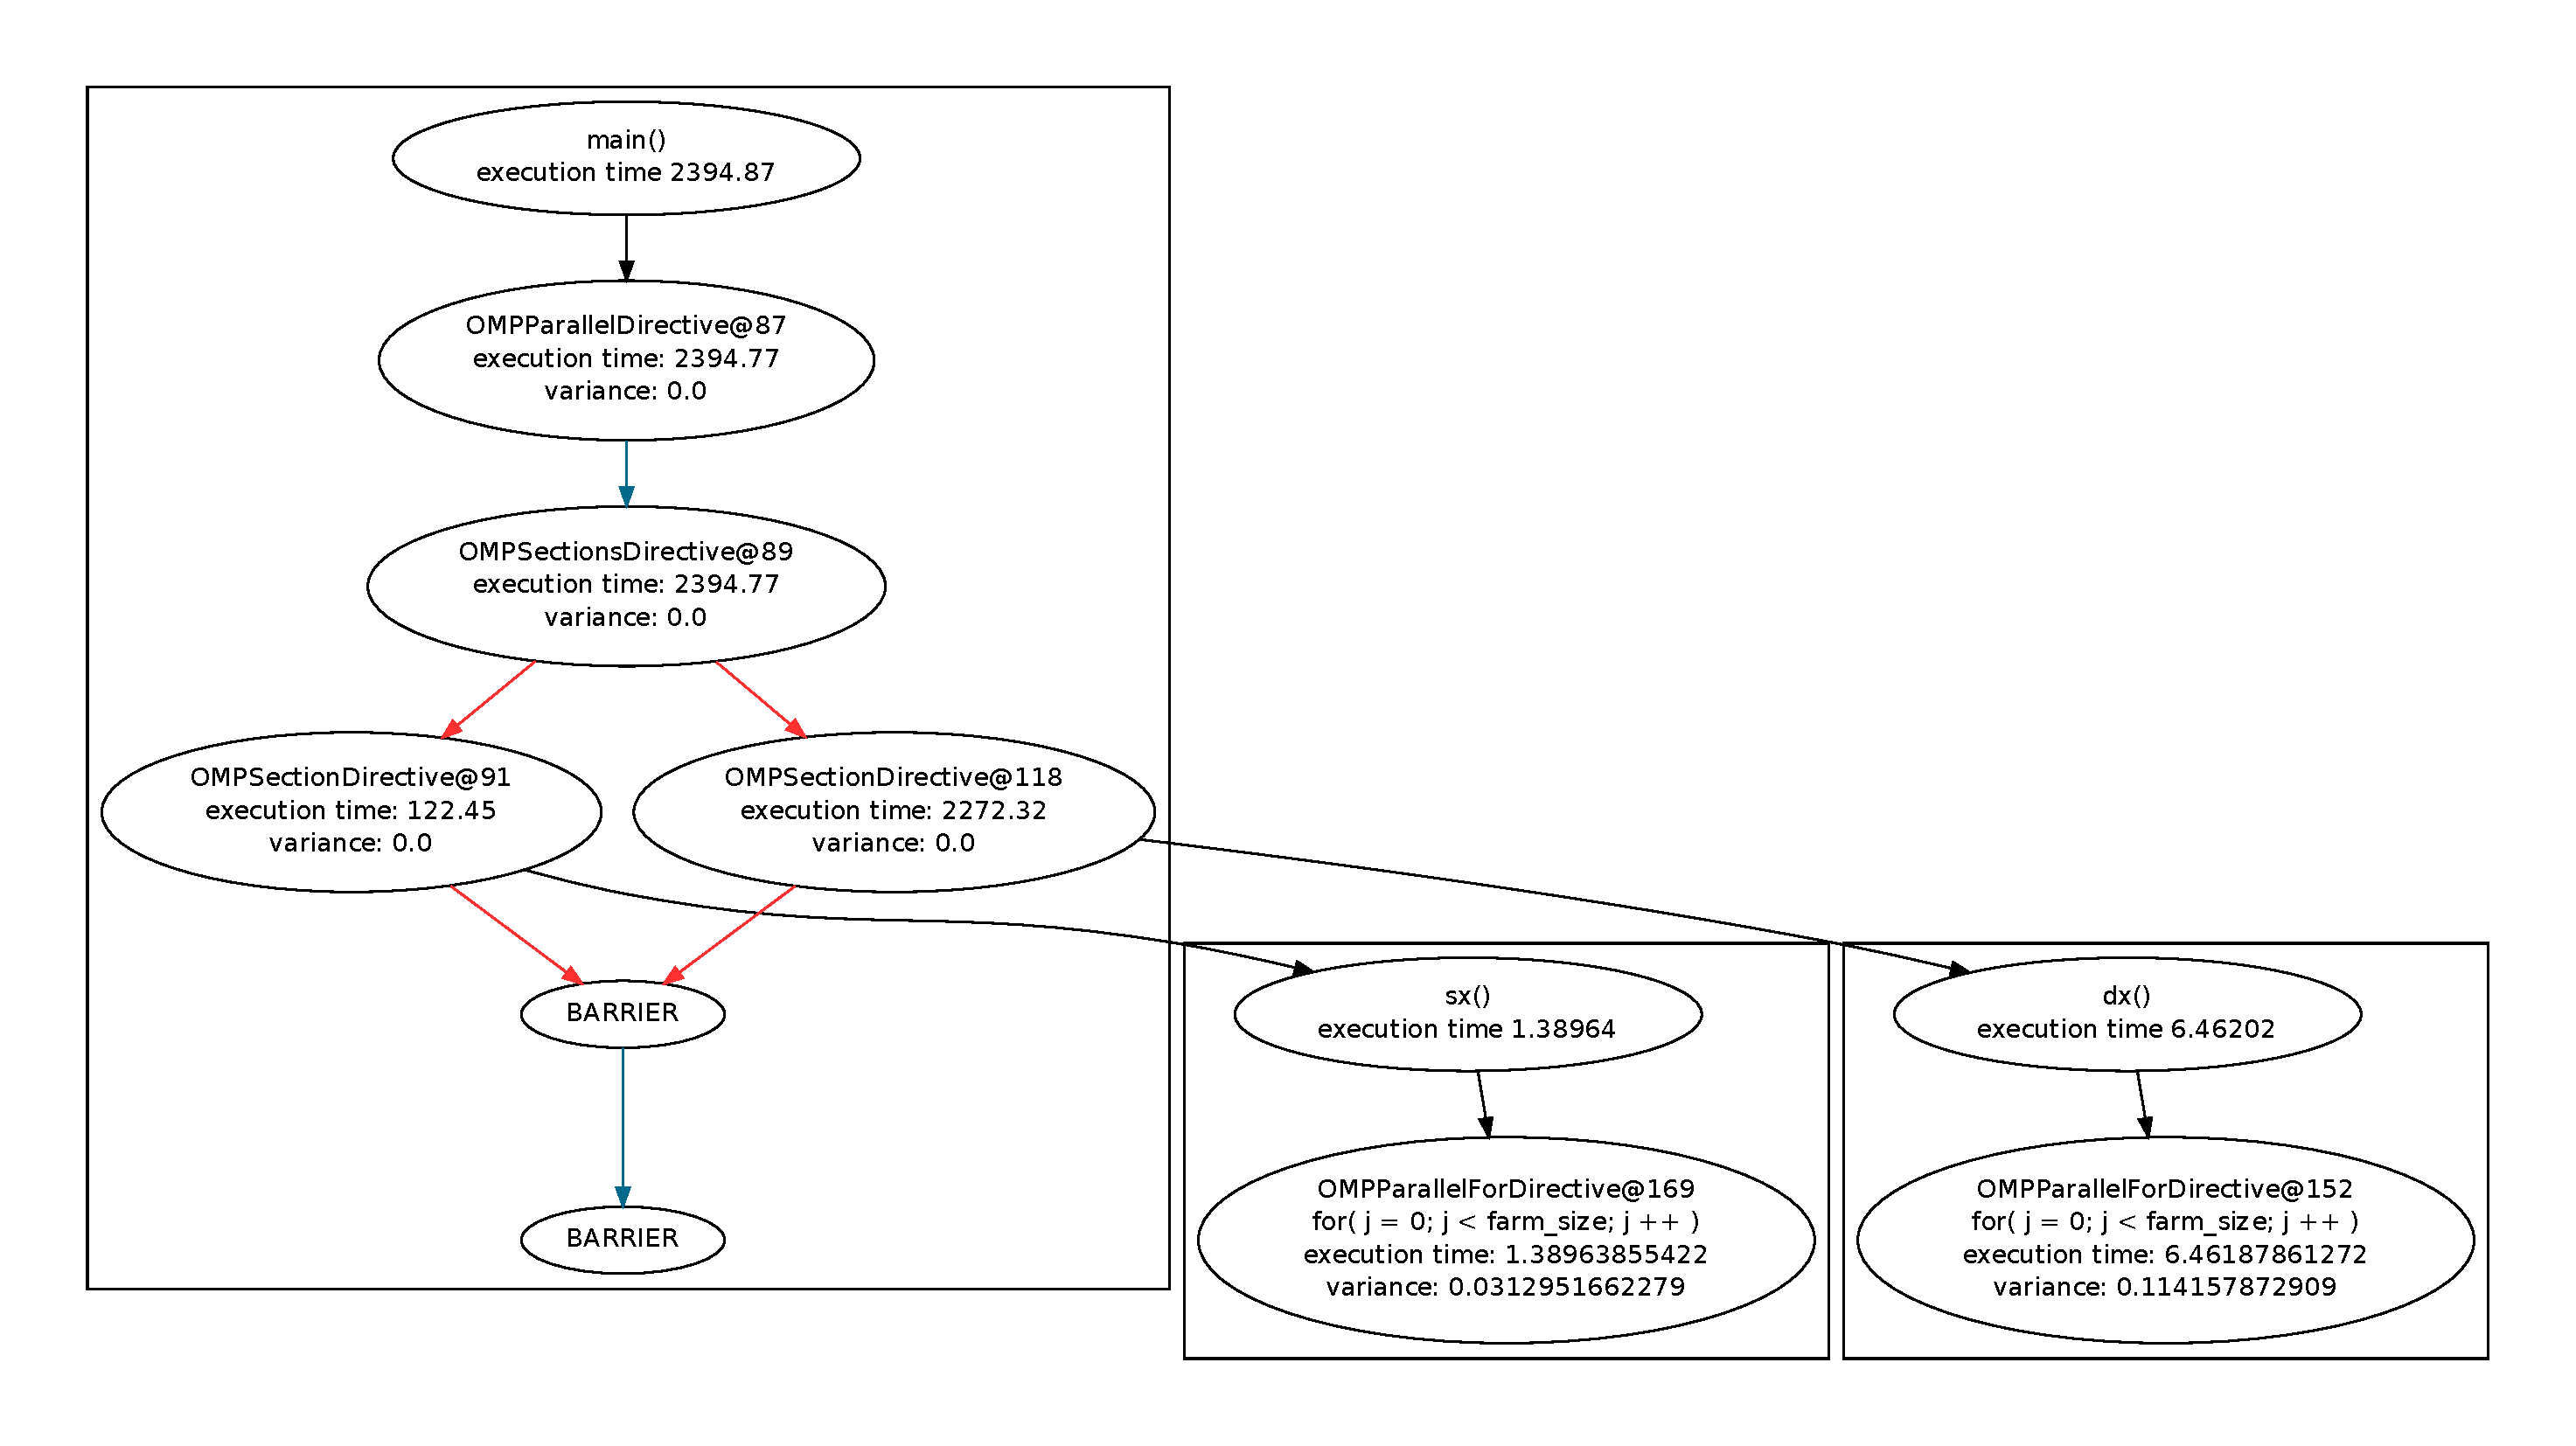
\includegraphics[scale=0.3]{functiongraphs.pdf}
\caption{Test structure.}
\label{teststructure}
\end{figure}

\section{Results with statistics}

\chapter{Conclusions}
\section{Achieved results}
\section{Future development}

The main future development step consists in the substitution of the OpenMP pragma directives with new self created pragmas in order to add new functionalities and simplify the framework. It could be possible, in principle, to add informations about deadlines, arrival times, schedule policies, \dots inside the directives. 

An interestin evolution would consist in adding a feature for specifying periodic task structures, which consist of a periodic activation time and deadline, directly in the pragma directives, either with or withou OpenMP. This is due to the fact that almost all \emph{real-time} programs consist of a majority of periodic tasks with some \emph{sporadic} tasks. The actual developed tool is already capable of executing periodic tasks, Code~\ref{periodictask}, by using an infinite for cycle with a timing control sequence nested inside which permits continuation or abortion.

\begin{lstlisting}[language=CCC, caption=Example of a periodic task., label=periodictask]
#pragma omp parallel for
for(...) {
	...
	work(); \\executes the periodictask
	wait(time); \\waits until the next activation time
	if(!continue) { \\checks the termination condition
		break;
	}
	...
}

\end{lstlisting}

The schedule algorithm could also be improved with better heuristics in order to obtain lower computation times for "good" schedule solutions. Another approach would consist in the parallization of the algorithm by taking care of race condition which would occur with the current used data structures.

The profiling step could extract more informations of the working platform to enhance the scheduling sequence and could check automatically different inputs to obtain the best results.

\begin{thebibliography}{30}
\bibitem{bbw2} G. Buttazzo, E. Bini, Y. Wu. \emph{Partitioning real-time applications over multi-core reservations}. Scuola Superiore Sant’Anna, Pisa, Italy, 2009
\bibitem{real1}J. Anderson, J. Calandrino, U. Devi. \emph{Real-time scheduling on multicore platforms.} Real-Time and Embedded Technology and Applications Symposium, 2006. Proceedings of the 12th IEEE. IEEE, 2006.
APA	
\bibitem{real2}B. Brandenburg, J. Calandrino,  J. Anderson. \emph{On the scalability of real-time scheduling algorithms on multicore platforms: A case study.} Real-Time Systems Symposium, 2008. IEEE, 2008.
\bibitem{tbb} C. Pheatt. \emph{Intel® threading building blocks.} Journal of Computing Sciences in Colleges 23.4, 2008.
\bibitem{ppl} D. Leijen, S. Wolfram, S. Burckhardt. \emph{The design of a task parallel library.} Acm Sigplan Notices. Vol. 44. No. 10. ACM, 2009.
\bibitem{boost} D. Abrahams, A. Gurtovoy. \emph{C++ template metaprogramming: concepts, tools, and techniques from Boost and beyond.} Pearson Education, 2004.
\bibitem{openmp} L. Dagum, R. Menon. \emph{OpenMP: an industry standard API for shared-memory programming.} Computational Science \& Engineering, IEEE 5.1, 1998.
\bibitem{icc} X. Tian, et al. \emph{Intel® OpenMP C++/Fortran Compiler for Hyper-Threading Technology: Implementation and Performance.} Intel Technology Journal 6.1, 2002.
\bibitem{parallware} http://www.appentra.com/appentra/parallware-auto-parallelizer-source-to-source-compiler/
\bibitem{realtimeopenmp}K. Lakshmanan, S. Kato , R. Rajkumar. \emph{Scheduling parallel real-time tasks on multi-core processors.}Real-Time Systems Symposium (RTSS), 2010 IEEE 31st. IEEE, 2010.
\bibitem{clang}http://clang.llvm.org/
\bibitem{llvm1} C. Lattner. \emph{LLVM: An infrastructure for multi-stage optimization}. Master Thesis, University of Illinois at Urbana-Champaign, 2002.
\bibitem{llvm2} C. Lattner, V. Adve. \emph{LLVM: A compilation framework for lifelong program analysis \& transformation}. International Symposium on Code Generation and Optimization, 2004. 
\bibitem{clanggcc}http://clang.llvm.org/features.html\#performance
\bibitem{rose} D. Quinlan. \emph{ROSE: Compiler support for object-oriented frameworks.} Parallel Processing Letters 10.02n03, 2000.
\bibitem{mercurium} J. Balart, et al. \emph{Nanos mercurium: a research compiler for openmp.} Proceedings of the European Workshop on OpenMP. Vol. 8. 2004.
\bibitem{intelomprtl}https://www.openmprtl.org/
\bibitem{clomp}https://github.com/motonacciu/clomp/
\bibitem{zvtm}http://zvtm.sourceforge.net/zgrviewer.html
\bibitem{mfp} Ricardo Garibay-Martinez, Luis Lino Ferreira and Luis Miguel Pinho, \emph{A Framework for the Development of Parallel and Distributed Real-Time Embedded Systems}
\bibitem{pop}Antoniu Pop (1998). \emph{OpenMP and Work-Streaming Compilation in GCC}. 3 April 2011, Chamonix, France
\bibitem{opencv}http://opencv.org
\bibitem{openbook}G. Bradski, A. Kaehler. \emph{Learning OpenCV: Computer vision with the OpenCV library}. O'reilly, 2008.

\end{thebibliography}

\end{document}